\chapter{Optical Imaging}
\label{apdx:optical_imaging} 

\section{From light to sight}

Objects are classified into 2 types: 
\begin{enumerate}
  \item luminous objects: ones that can generate their own light (e.g. the sun,
  the street light, the table lamp)
  \item illuminated objects: one that are capable of reflecting lights coming
  from luminous objects.
\end{enumerate}
The coming light is called {\bf incident light}. If the light pass through the
object and change  the direction, it's called the {\bf diffracted light}. If the
light is reflected, , it is called {\bf reflected light}.

The {\bf law of reflection} states that ``angle of incidence and angle of
reflection is the same'', Fig.\ref{fig:light_angle} (A).
This is true when the surface of the illuminated object is a plane (mirror) and
the surface is mooth. So, the type of reflection is known as {\bf specular
reflection}. What if the surface is rough, which is true at the microscopic
level? Indeed, the bundle of parallel incident lights become defracted and
diffuse in different directions; known as {\bf diffuse reflection},
Fig.\ref{fig:light_angle}(B). 

A human's eyes can 'see' an illuminatable object when the reflected light
projected into human's eyes. Standing at different angle of the incident light,
we can sense an object differently (brighter/darker, smaller/larger). Depending
on the quality of reflected light, we can see clearly, or not seeing it at all.
In the dark, we cannot see anything. In a dim light, we can see an object
blurry. The main source of light is the sun.
Lights from the sun is colorless.

\begin{figure}[hbt]
  \centerline{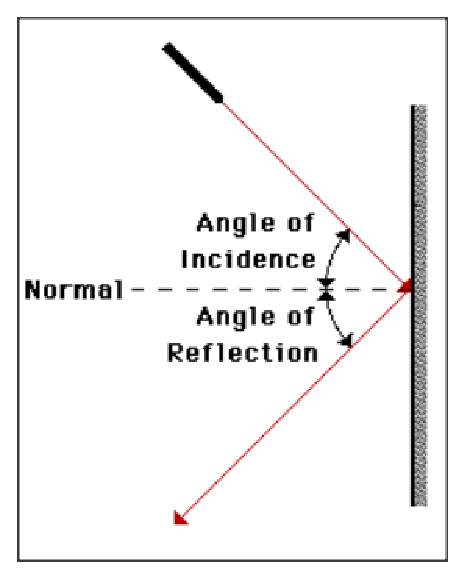
\includegraphics[height=4cm,
    angle=0]{./images/light_angle.eps}
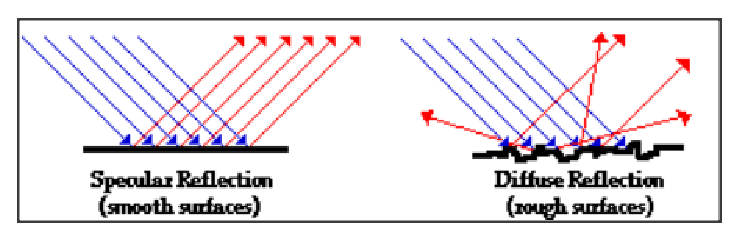
\includegraphics[height=3cm,
    angle=0]{./images/light_diffuse_reflection.eps}}    
\caption{(A) Incident/Reflected light and angles; (B) Specular and Diffuse
reflection }
\label{fig:light_angle}
\end{figure}

% So,
% it's the light coming to the object, then reflected onto the human eyes,
% allowing our human eyes to sense objects. 

\begin{framed}
In order to perceive an object, we need 'visible' lights and then the human
indeed perceive the object via the reflected light. If the object absorb the
light completely, i.e. there is no reflected light, the object become invisible
under human eyes. Human eye can sense the light with wavelength in the range
380nm to 760nm. Lights with wavelengths in this range are 'visible' lights, and
their colors, in the order of increasing wavelength, are violet, indigo, blue,
green, yellow, orange, and red. 
\end{framed}

The wavelength of the light determines the light's color and the energy of the
lights. Indeed, the sun light is composed of lights of different wavelengths.
Some of the wavelengths are visible to human eyes, and some are not. Each
visible wavelength when reaches the human eyes are perceived as some different
colors.

\section{Telescope vs. Microscope}

If the object is too far away or too small or the incident light is weak,
there's not enough reflected light coming to the eye. That's why a naked eye
cannot see these objects. To help naked eye seeing object from far away, we need
some device to collect more reflected light from the object, and bring that
light to a point of focus (on the retina of the human eye) by the cornea and
lens of the eye.

\begin{enumerate}
  \item Telescope: we use if the object is TOO FAR away. There're 3 types of
  telescope:
  {\bf refractor} that use lens to collect lights, {\bf reflector} that uses
  mirror to collect lights, and the compound (combination of both).   It's the
  {\bf objective lens} (in refractors) or {\bf primary mirror} (in the
  reflector) that collects the light and bring to a focal point. The eyepiece
  lens in the refractor is placed near the focal point and takes the bright
  light from the focus and 'spread it out' (i.e. magnify it to take up a larger
  portion on the retina).
  
\begin{framed}
INTERESTING FACTS: When looking at the stars or objects in the sky, we don't
want to use large magnification (i.e. low power as 50x is enough). What we need
is the telescope to bring more lights, not to magnify the object that much. The
light-gathering capability is directly related to the size of the primary lens
or mirror.
\end{framed}  

  \item Microscope: we use if the object is TOO SMALL. A microscope need a
  special light-source, and a {\bf condenser} to focus the
light from the source onto a tiny, bright spot of specimen. Unline the
telescope,
  there is no need for a large objective lens; the objective lens is small and
  spherical (so that it can bring the image of the small object into focus at a
  short distance). The image on the focus is magnified by a second lens ({\bf
  eyepieces} or {\bf ocular lens}).
\end{enumerate}
 
In a microscope, factors that affect the quality of an image?
\footnote{\url{http://science.howstuffworks.com/light-microscope2.htm}}
\begin{enumerate}
  \item brightness (how light or dark of the image): the more light (i.e.
  brighter image) can be achieved by increasing N.A. of the objective lens (the
  larger, the brighter), or adjusting condenser.
  
  \item focus (blur or well-defined image): adjust the focal length.
  
  \item resolution (how closed two small objects can be identified as two
  separate objects): adjusted by N.A. (higher N.A., the better resolution), and
  choosing the proper wavelength (the shorter the better) 
  
  \item contrast: the ability to distinguish an object from the background
\end{enumerate}

A main problem with observing specimens under the microscope is that their
images do not have much contrast, especially true for living things (e.g.
cells). To resolve this issue and to be able to detect certain subcellular
structure, the pigment or dyes (probe, fluorescent) that bind to that specific
structure within the specimen is used. Fluorescence is a popular type of dye
being used to measure level of specimen (e.g. calcium).  The laser light is then
projected into the specimen, and the proper wavelength to be reflected when
coming to the pigment-bound specimen is detected and recorded. More detail of
microscope, read Sect.\ref{sec:microscope}.


\section{Classification of microscope}
\label{sec:microscope}

The smallest object an unaided human eye can see is about 0.22 mm in diameter,
Fig.\ref{fig:scale_life}.
\url{http://learn.genetics.utah.edu/content/begin/cells/scale/}

\begin{figure}[hbt]
  \centerline{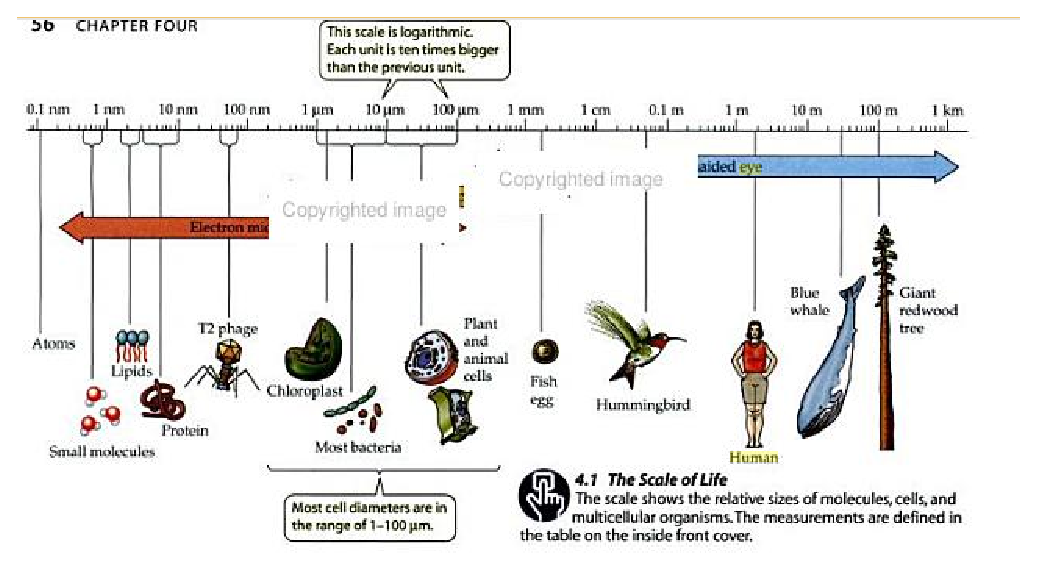
\includegraphics[height=5cm, angle=0]{./images/scale_life.eps}}
  \caption{The scale of life\citep{purves2001}}
  \label{fig:scale_life}
\end{figure}

A microscope is a device that help us to see objects too small for the naked
eyes by magnifying the image. The first available microscope is the one that
redirect the visible light, while the later ones use novel technologies.
Depending on its use, microscopes are classified into 3 types.

\subsection{detect objects: optical microscope, electron microscope, immunoEM}

This first type is to discriminate objects
\begin{enumerate}
  \item optical (light) microscope (since 16th century): use visible light
  (400-700 nm). The smallest thing to see is limited by the wavelength. So, with
  the shortest visible wavelength of 500nm, the smallest thing we can see is
  500nm in diameter. The most powerful light microscope can resolve bacteria,
  but not viruses. To see anything smaller than that, we need electron
  microscope. 

  \item electron microscope (since second world war): use electrons, rather than
  light, to generate the image, and electromagnets instead of glass lenses. It
  shoots a high voltage-beam of electrons onto or through an object which can
  deflects or obsorbs some of the electrons. The resolution is limited by the
  wavelength of the electrons beam which can resolve molecules or even
  individual atoms. 
\end{enumerate}

ImmunoEM (Immuno-electron microscopy) refers to the technique of detecting the
presence of a particular protein; via immunostaining
(Sect.\ref{sec:immunostaining}) to study the detailed microarchitecture of
tissues or cells.
While powerful in detecting the sub-cellular localisation of a protein,
immuno-EM can be technically challenging, expensive, and require rigorous
optimisation of tissue fixation and processing methods.



\subsection{visualize surface: scanning probe microscope, atomic force
microscope}

The second type of microscope, not to discriminate objects, but to visualize the
surface of small objects
\begin{enumerate}
  \item scanning probe microscope (since 1981): using physical probe (very
  small in size) that interact with the specimen, recording the probe-surface
  interaction, i.e. ``feeling'' the surface of the one we want to measure. The
  probe tip is often made of platinum/iridium, gold, etc. 
  \item atomic force microscope
  \item \ldots
\end{enumerate}

\subsection{measure density (concentration): fluorescence microscope}

\textcolor{blue}{The third type of microscope, to measure the density
(concentration) of a specimen, which is being widely used in life science}
\textcolor{red}{[We will focus on this type]}. The principle is that a certain
material can emit energy under a visible light. This energy reaction only occur
at a particular wavelength for  a given material.

\begin{enumerate}
  \item fluorescence microscope (last decade of 20th century, use in
  biology):  use much higher intensity light source to excite a fluorscent
  species which in  turns emits a lower energy light of a longer wavelength.
  This reflected light is detected to generate the image. An example: the
  electron emits green light when stimulated with blue light.
     
 \item better resolution: by reducing PSF anistropy in 3D 
 \begin{itemize}
   \item pupil filters: narrower PSF main peak at the expense of higher
   sidelobes (in conventiional imaging, but not in confocal imaging, especially
   bright-field confocal microscopy\cite{martinez-corral2003}). The method
   doesn't work well with single-photon fluorescence confocal microscopy due to
   undesired photo-bleaching.
     \item 4Pi microscope:    
  \item breaking the diffraction-limit, Fig.\ref{fig:diffraction_limit}: STED,
  PALM/STORM and TIRF microscopes
 \end{itemize}
\end{enumerate}

\begin{figure}[hbt]
  \centerline{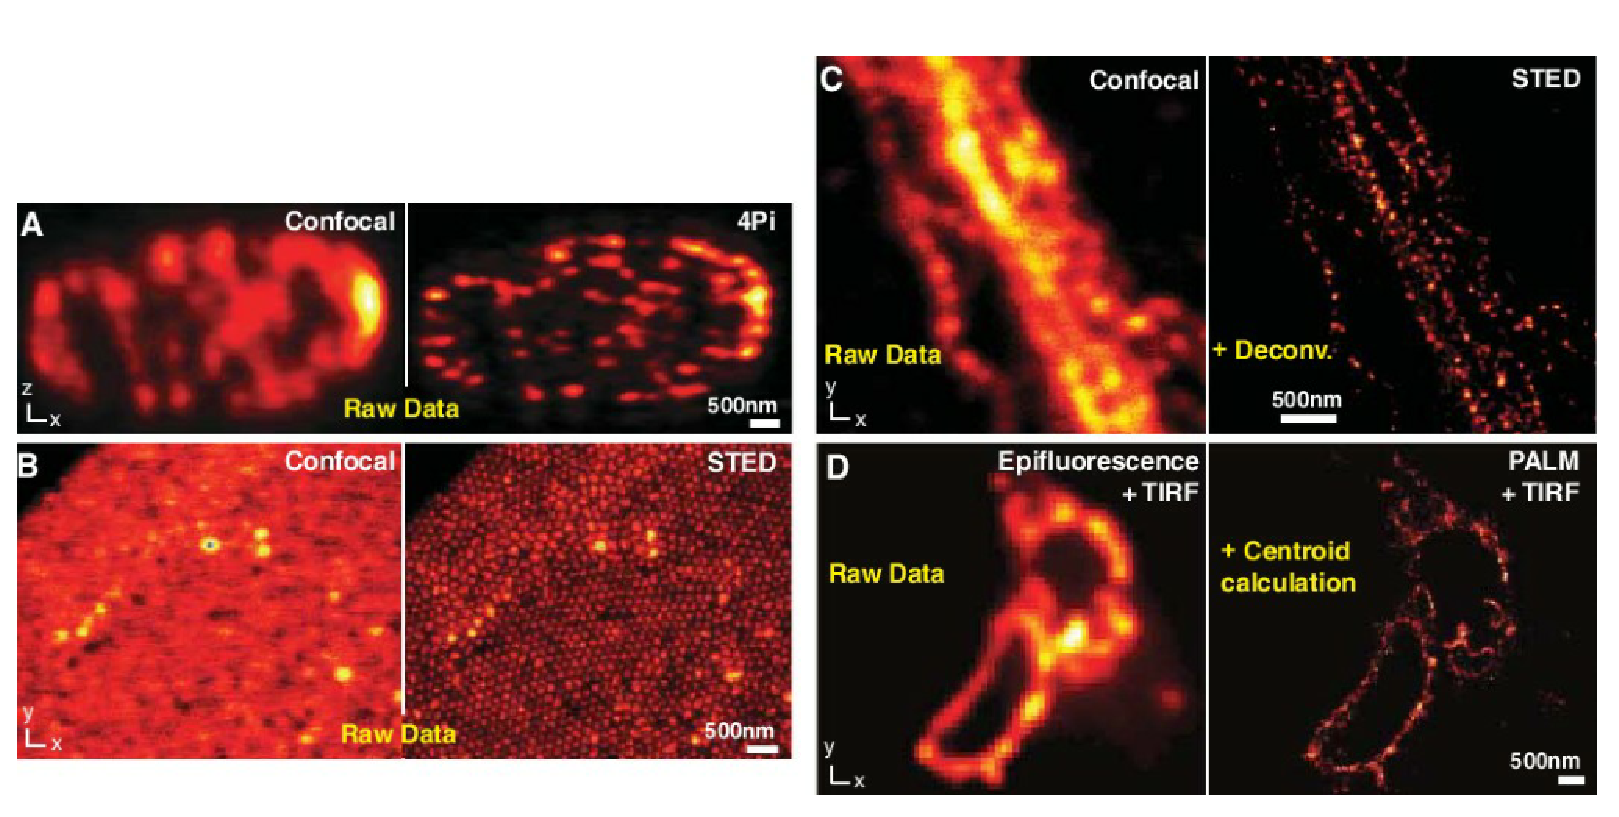
\includegraphics[height=5cm,
    angle=0]{./images/diffraction_limit.eps}}
  \caption{Breaking the diffraction limit}
  \label{fig:diffraction_limit}
\end{figure}


\textcolor{red}{We'll focus on fluorescence microscope}
(Sect.\ref{sec:fluorecence_microscope}). In calcium imaging, fluorescent
molecules after binding to calcium, changes their fluorescent properties. The
fluorescence when binding to the specimen generate a different difracted
wavelength. We choose the light so that only the calcium-bound fluorescence
absorb the light, but not the free fluorescence. Typically, the binding is
assumed 1 $\Ca$ ion : 1 fluorescence molecule. So, depending on the intensity of
the difracted wavelength, we can estimate the concentration of the specimen.
    
  \begin{itemize}
    \item epifluorescence microscope (EFM):
    \url{http://cse.lmu.edu/resources/MANE_Labs/Instruments/Epi-fluorescence_Microscope__EFM_.htm}
    \item confocal microscope:
    \item multi-photon
    \item single-photon
  \end{itemize}

% A widely used terminology is {\bf resolution}: which refers to the capability of
% a microscope giving a human eye to distinguish two small objects closed to each
% other. 


% \subsection{Light microscope}
% \label{sec:light_microscope}

\subsection{correlated light microscopy and EM (CLEM), aka correlative light
microscopy and EM}
\label{sec:correlative-microscopy}

correlated light microscopy and EM (CLEM) is the imaging technique that bridge
electron microscopy (EM) and fluorescence microscopy.

Despite the power that enable us to 'see' molecules via fluroescence, still a
large fraction of molecules remain unlabeled and therefore 'in the dark', the
context of the localization is lost.
Also, the resolution of light microscopy (LM) is typically submicrometer and
thus does not match the size of biomolecules, which typically range from 0.1 to
10 nm. EM can help with this; but its result is based on grayscale images; and
yet the samples are in fixed state; so  finding rare events in space and time is
nearly impossible.

Using CLEM, it enables the study of a rare  cellular 
(or subcellular) events in their cellular context. 

\section{Fluorescence microscope}
\label{sec:fluorecence_microscope}

Imaging {\it in vivo} or {\it in vitro} ion concentration such as calcium
using fluorescent calcium indicator is parallel with the development of
different imaging techniques.
\begin{itemize}
  \item  video imaging (Smith and Augustine, 1988; Swandulla et al., 1991), 
  
  \item CCD cameras (Connor, 1986; Lasser-Ross et al., 1991), and 
  
  \item high-speed confocal microscopy (Eilers et al., 1995) for calcium imaging
\end{itemize}

A conventional fluorescence micrscope is the one equipped with a high-intensity
light source (e.g. mercury arc lamp) that emits light in a broad spectrum from
visible to ultra-violet wavelengths.

Mellors and Silver developed the concept of fluorescence microscope in 1951
\citep{mellors1951}. When a light incident on a molecule; the electrons
in the molecule can absorb the light and then emit light of a different color
(i.e. different wavelength). This process is known as {\bf fluorescence}. Minsky
in 1957 developed and designed confocal microscopes \citep{minsky1957}, yet it tooks
another thirty years for the first commercial laser confocal microscope to be
developed (review:\citep{pawley2006}). Since then, there are several advances in
technology: 
\begin{enumerate}
  \item  wide-field microscopy, 
  
  \item one-photon, 
  
  \item multi-photon (e.g. two-photon) introduced in 1990 -
  Sect.\ref{sec:two-photon-confocal-imaging}, and
  
  \item multicolor.
\end{enumerate} 

\begin{framed}
At normal temperature, most electrons in a molecule stay at the ground state
(lowest energy state). When the electron absorbs a photon, it may jump to a
discrete new energy state (excited state). It then quickly (within $10^{-8}$
sec) loose some of its energy to neighboring molecules when colliding them or
releasing as heat due to vibration. The left over energy is released when the
electron emit in the form of photon of longer wavelength, so that the electron
can goes back to the ground state. 
\end{framed}

The charge coupled device (CCD) cameras can detect fluorescence in the
ultraviolet (UV) and infraed (IR) range. In biological confocal microscopy,
however, visible lights as difracted lights are widely used,
Fig.\ref{fig:visible_lights}. NOTE:
\textcolor{blue}{Indigo is not well differentiated from violet by human eyes.
Near-UV light (300-380nm) is useful in fluorescence microscopy primarily as the source of
excitation photons; while near-IR lights (750-1400nm) are useful in multi-photon
excitation}.

\begin{figure}[hbt]
  \centerline{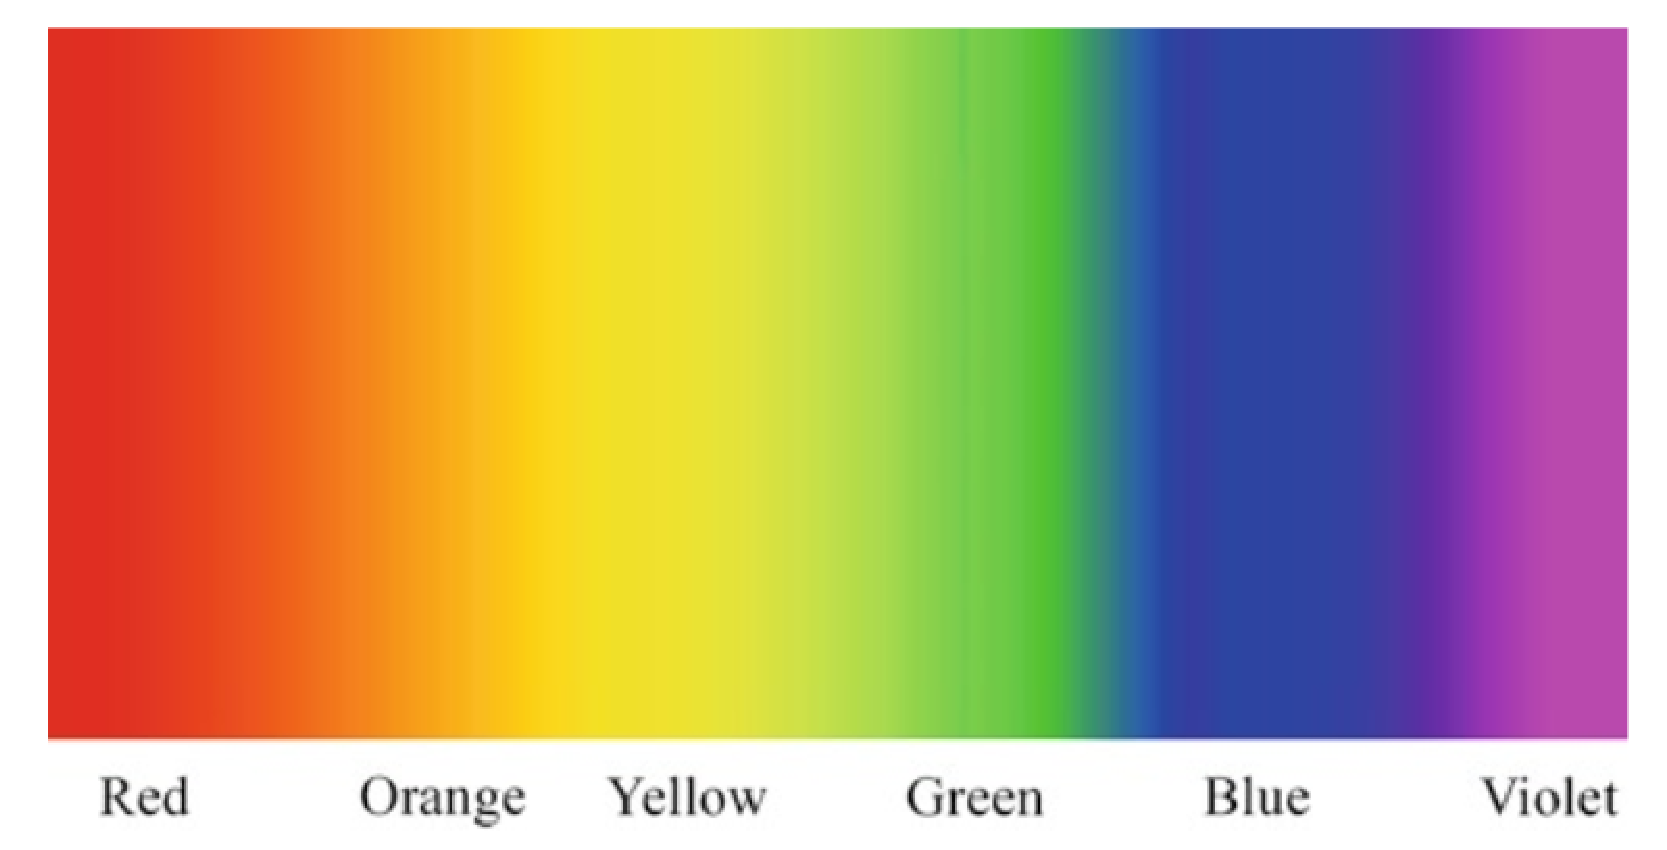
\includegraphics[height=3cm,
    angle=0]{./images/visible_lights.eps}}
  \caption{Range of visible lights (from 380nm to 750nm) with red(620-750nm),
  orange (590-620nm), yellow (570-590nm), green (495-570nm), blue (450-495nm),
  indigo (425-450nm) and violet (380-425nm)}
\label{fig:visible_lights}
\end{figure}



\subsection{Resolution limit: Wavelength ($\lambda$) and Numerical Aperture
(N.A.)}
\label{sec:resolution_limit}

An optical microscope produces a magnified image of a small object. During the
imaging process, emitted light rays from each point on the object maps to a
single pixel on the image plane. Due to the diffraction limit, in the confocal
microscope, a point-like light source produces an electromagnetic field on the
image plane. This field is commonly represented through {\bf amplitude  point
spread function}. Actual specimens are not point sources, but can be  intepreted
as a superposition of an infinite number of objects having dimensions  below the
resolution of the system. So, instead of a sharp spot, the image of a single
spot on the object is showed as a 3D gaussian intensity distribution image,
known as a point-spread function (PSF). The size of the PSF determines the
resolution of the microscope. It means that if two objects with the distance
shorter than the FWHM of the PSF, the microscope will be difficult to resolve
them (Sect.\ref{sec:PSF}).

The ability to distinguish two adjacent objects depends on the wavelenght
$\lambda$ of the reflected light, and the numerical aperture (N.A.) of the
objectives (i.e. the lens). Ernst Abbe (1873, 1884) pointed out that
the diffraction of light (1) by the specimen, and (2) by the objective lens
determine the resolution of the projected image. From that, it was established
the role of objective and condenser {\bf numerical apertures} (NA) on image
resolution. 

The distance limit or the minimum distance for the two objects be resolvable is
\begin{equation}
R = \frac{0.61 \lambda}{\text{N.A.}}
\end{equation}
% so $\lambda=480$nm, then $R\approx 0.2\mum$. Cell structures can be of size
% smaller than this.

Numerical Aperture (NA) reflect the light cones with respect to the change in 
angular aperture $\alpha=2\theta$
(example:\url{http://micro.magnet.fsu.edu/primer/java/nuaperture/index.html}).
So, {\bf numerical aperture} (N.A.) (hardware: objective lens) refers to the
capability to gather light, and {\bf magnification} (hardware: eyepiece) refers
to the ability to enlarge an image.

\begin{figure}[hbt]
  \centerline{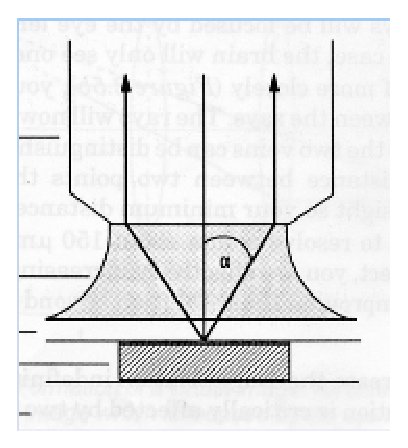
\includegraphics[height=3cm,
    angle=0]{./images/NA_microscope.eps}}
  \caption{The objective lens catch the refracted lights with a maximum angles
  $\alpha$}
  \label{fig:NA_microscope}
\end{figure}

Given $\alpha$ is the angle of the cone of light (accepted by the objective lens
$\alpha_\text{obj}$ or emerged from the condenser lens $\alpha_\text{cond}$),
$\eta$ is the refractive index of the medium between the specimen,
Fig.\ref{fig:NA_microscope}, the (objective NA$_\text{obj}$ and condenser
NA$_\text{cond}$) lens is calculated as
\begin{equation}
\text{NA} = \sin (\alpha/2) \eta 
\end{equation}

Theoretically, the highest angular aperture is 180$^\circ$. A majority of light
microscope is designed to work with air, where $\eta = 1.0$.
So, in air (dry objective), the theoretical maximum NA is 1.0. In practice, the
highest value is 0.95 (with the half angular aperture is 72 degreees). In oil,
oil immersion objectives can achieve much higher N.A. In oil media,  $\eta$ is
typically 1.52. The bigger N.A., mathematically, the increase in the angular
aperture; and practically, the more light can be captured, giving brighter and
higher resolution of the image at a fixed magnification. However, the higher
N.A., the more noise is captured as well.

NOTE: $\eta=1.32-1.34$ (water), $\eta=1.44$ (glycerul 75\%), $\eta=1.36-1.5$
(protein), $\eta=1.5-1.6$ (nucleic acids).


{\bf contrast}, defined for two objects of equal intensity, is defined as the
difference between the maximum intensity and the minimum intensity of the space
between the two objects. The maximum intensity of the Airy disk is normalized,
so the maximum of contrast is 1 and it happens when the distance of the two
objects is relatively large. The value of contrast tell how easily to
distinguish the two objects. 

There is a minimum distance at which the peak of the two objects are
indiscernible if the distance is shorter than this value. This is known as {\bf
contrast cut-off distance}. However, for the two point-sources to be visually
distinguishble, a well-known criterion {\bf Rayleight criterion} is stated that
{\it two points are resolved when the first minimum  (zero-crossing) of one Airy
disk is aligned with the central maximum of the second Airy disk}. This distance
is calculated as (in wide-field microscope)
\begin{equation}
r_\text{lateral} = 1.22\lambda/(2.\NA) = 0.6\lambda/\NA
\end{equation}
with $\lambda$ is the emitted light wavelength, NA is the numerical aperture of
the objective. This maps to the distance with contrast value 26.4\% (at optimum
imaging condition). 

As measuring the maximum of the Airy disk is hard, the minimum distance is
typically calculated using the FWHM of the PSF. However, the calculated value is
somewhat smaller than the valued calculated from Rayleigh criterion. 

So far, we're talking in the analog sence, with continuous function. The fact
that all digital confocal microscopy images are acquired, processed, and
displayed in the realm of discrete partitions requires us to consider the effect
of choosing the smallest spatial element called {\bf resel} (pixel, voxel), the
smallest area that can be distinguish from the neighboring area.  

Sampling criterion refer to the sampling interval in space and time that is
required to reproduce features of interest with sufficient contrast is relied
upon the well-known {\bf Nyquist criterion}. For the  since wave, Nyquist found
that to reconstruct it, we need at least twice sampling during each cycle of the
wave (that is in time). For spatial data, it's 2.3 times the maximum frequency
to be reconstructed. The pixel size should be smaller than the inverse of the
2.3times the cut-off frequency
\begin{equation}
\text{Pixel size} < 1/(2.3f_\text{cut-off})
\end{equation}

\subsection{Fluorescent probe	}

\begin{framed}  

  A fluorescent molecule or fluorescent protein  is something that glows a
  visible color when exposed to certain light (typically, ultraviolet light).
  The mechanism is that the incoming light raise the energy of the electrons in
  the fluorescence molecule to an excited state. The electrons then vibrate and
  then returns to the ground state, along with release some energy in the form
  of emitted light. NOTE: The released energy is not the same as the absorped
  energy as during vibration, some was lost as heat. The lost energy is known as
  non-radiactive energy. So, the incoming light should have the highest energy
  and the wavelength should be higher than the visible wavelength, which
  explains why the ultra-violet light is often used. Beside, the light need to
  be absorped, so both absorption and higher energy are required. It means that
  a dye absorp lights from a certain range of wavelengths.
\end{framed}  

The electrons in a fluorescent molecule absorb a photon of light of a particular
wavelength, which brings the electron to a new unstable energy level before it
completely release the energy to switch to the stable ground state.
The delay in emission, i.e. the time from reaching activated state, vibrating
and then releasing the photon light to return to the ground state, is called the
{\it fluorescence lifetime}. The emitted energy is not the same as the absorbed
energy as a fraction of this energy is lost due to molecule movement, friction,
etc. This difference in energy is called {\bf Stokes' shift}. Since the emitted
photon has less energy, it has a longer wavelength, i.e. a different color than
that of the absorbed photon.
However, the degree of shift is highly dependent upon the molecule being
excited, i.e. the type of fluorescence probe, e.g. Cy3 has wavelength difference
is 14 (incoming wavelength 548nm, and emitted wavelength 562nm). Of course, the
emission and excitation do not occur at a single wavelength, but at a range.
However, there's a higher probability to emit at one wavelength than another,
and similarly with excitation, Fig.\ref{fig:emit-excite_TRITC}. The larger the
separation, the better the filter of the excitation light from the emitted
light, giving the better image quality.

\begin{figure}[hbt]
  \centerline{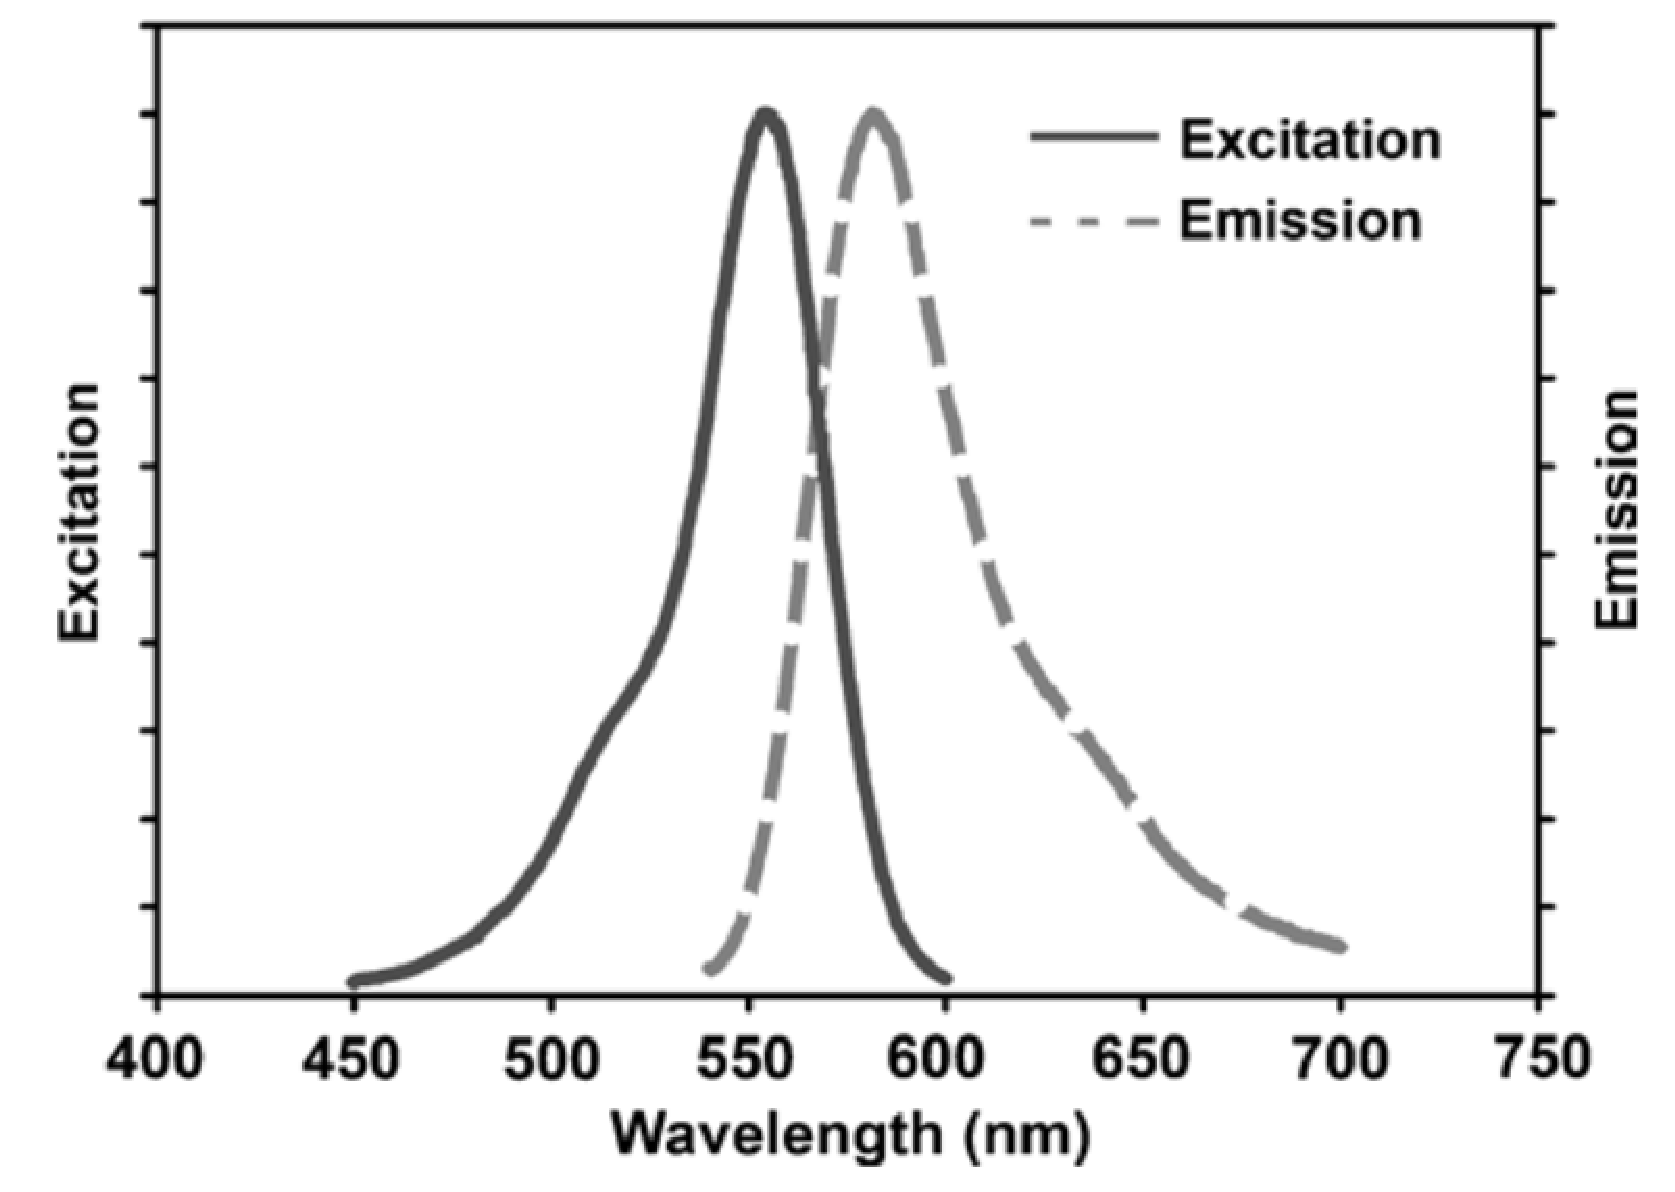
\includegraphics[height=4cm,
    angle=0]{./images/excite_emit_TRITC.eps}}
  \caption{Excitation and Emission spectra for TRITC}
\label{fig:emit-excite_TRITC}
\end{figure}

In a cLSM, a fluorescent probe when binding to the specimen, absorbs a single
photon at one wavelength, enters the excited state for a short period of time,
before emitting the photon at a longer wavelength. A significant disadvantage of
fluorescence is the occurrence of {\bf photobleaching} or fading. Bombarding
fluorescent probe with high-energy illumination at the optimal excitation
wavelength can damage their chemical structure. Also, at the excited state,
fluorescent probe can also form covalent association with other molecules,
decreasing fluorescence capacity. To avoid photobleaching, a novel technique
using discontinuous light is used, giving the name {\it multiphoton microscopy}.

To be able to detect multiple targets, multiple synthetic dyes are used at once.
These dyes need (1) avoid spectral overlap, (2) high quantum yield, (3) stable. 

Nowadays, GFP (green fluorescent proteins) are used as these proteins are used
to construct fluorescent chimeric proteins that can be expressed in living
cells, tissues, and entire organisms, after transfection with engineered
vectors. The current problems with many dyes:
\begin{enumerate}
  \item most are oligomeric, so it can cause problems {\it in vivo}
  \item most are red proteins, i.e. not usable in the red-far region
  \item large size (20-30 kDa), so insertion tag may affect location/function of
  tagged target protein.
\end{enumerate}


\subsection{Light source}
\label{sec:light_source}

There are three options for lightsrouces: 
\begin{enumerate}
  \item Mercury or Xenon lamps: excite with variable intensities
  \item LEDs: long lasting, with variable power and different wavelengths
  \item laser (gas/solid state): high-intensities monochromatic light source,
  use with limited number of wavelengths.
\end{enumerate}

Mercury lamp produces photons with wavelengths cover the full visible spectrum
and UV range. However, mercury arc lamps show peak intensities at 313nm, 334nm,
365nm, 406nm, 435nm, 546nm, and 578nm. At other wavelengths, the intensities are
much lower, Fig.\ref{fig:light_source}(A). 

Xenon lamp has a more uniform distribution of intensities across the visible
range, but the intensities drop off rapidly at UV-light, i.e. wavelength below
400nm, Fig.\ref{fig:light_source}(B). 

\begin{figure}[hbt]
  \centerline{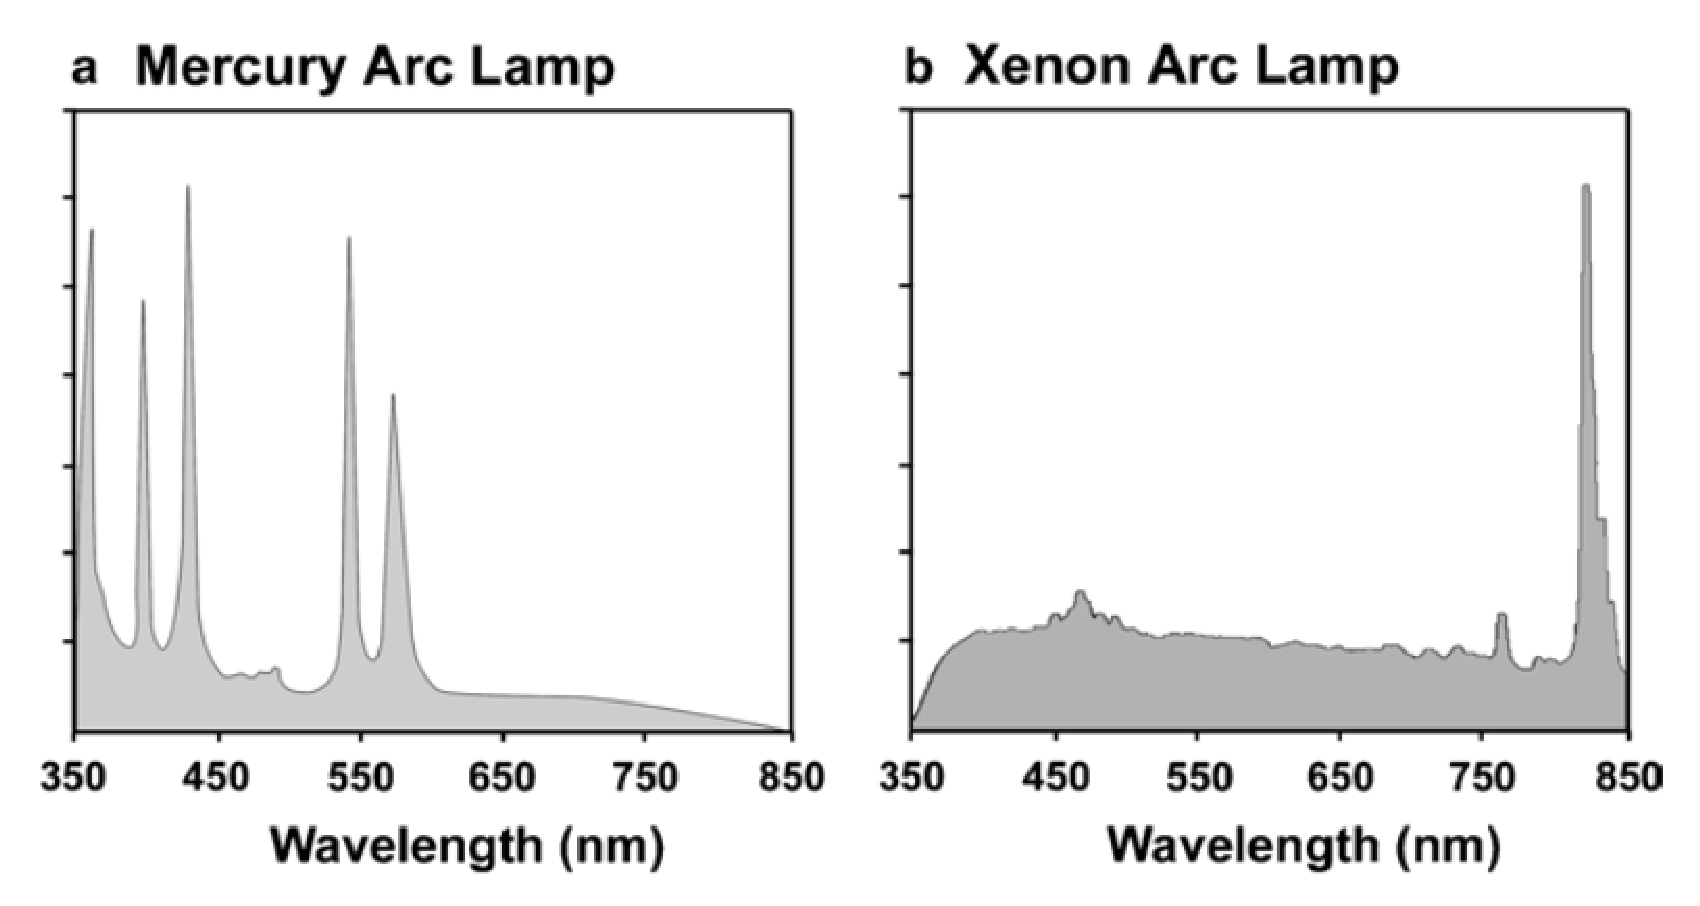
\includegraphics[height=4cm,
    angle=0]{./images/light_source.eps}}
  \caption{Spectrum of light emitted from mercury and xenon arc lamps}
\label{fig:light_source}
\end{figure}

The intensity light sources are Xenon or Mercury arc-discharge
lamp\footnote{\url{http://serc.carleton.edu/microbelife/research_methods/microscopy/fluromic.html}}.
The drawback of mercury and xenon lamps are short lifespan, instability, and
unwanted wavelengths to be excited. New light sources are high-performance LEDs
(light-emitting diodes) that produces high and stable output, long usuable
lifespan, with less heat and very low energy consumption. The drawback of LEDs
is the less intense output. With LEDs, light can be produced with a narrow
wavelengths, making it easier to filter out unwanted wavelengths.

Using point-to-point illumination, at a single time instant, only a few emitted
photons can be collected. Thus to avoid noise, each point must be illuminated
for a long time enough to collect enough photons for making an accurate image.
This may cause the problem of lower temporal resolution, i.e. it takes long time
to generate an image. The solution is to use light source with very high
intensity. The modern choice is laser light (i.e. {\bf laser confocal
microscope}). 

The use of fluorophore as the dye has its own weakness; fluorophore loose its
ability to fluorescences in a process called {\bf photobleaching}. The short
wavelength being used also damange the fluorecent. Also, there's a limit of the
resolution given the smallest wavelength that can be focused (technologically,
it's called {\bf diffraction limit}). The limit is mathematically formularized
with about half of the wavelength of the light used. \textcolor{red}{We will
see how the newer techniques overcome these limitation, especially the
diffraction limit}.

\begin{framed}
The wave-like character of diffracted light prevents objects smaller than
approximately 200nm in laterl (x,y) and approximately 500nm (in z-dimension)
from being visualized as anything but blur. 

There are many subcellular structures smaller than this limit (e.g.  actin
fibers, intermediate filaments, microtubules, ribosomes, and transport
vesicles). Thus, imaging beneath the diffraction limit is a challenging (See
Sect.\ref{sec:STED}, \ref{sec:PALM}).
\end{framed}

\subsection{Detector CCD cameras}

There are different CCD cameras with different resolutions:
\begin{enumerate}
  \item Axiocam HRc (colour): 1.4 MP (1388x1040 pixels in the size
  6.45x6.45$\mum$) with frame rate 5 fps (20ms exposure)
  
  \item Olympus DP71: 1.45 MP, coupled with pixel-shifting technology, giving
  ultra-high resolution 4080x3072 pixels.
  
  \item FVII: 1376x1032x6.45$\mum$ square pixel CCD monochrome imaging sensor
  that gives high frame-rate 22 fps or 30 fps with binning.
\end{enumerate}

Newer cameras use electron multiplying CCD (EMCCD) cameras technology. It can
amplify weak signals (down to single photons) to a signal level that is well
clear of noise, at any read-out speed. 
\begin{enumerate}
  \item iXon +885 camera: high resolution with high QE at 32 fps.
  \item iXon +897 camera: single photon detection capability without image
  intensifier. It delivers 512x512 pixel frame (16$\mum$ square).
\end{enumerate}
The EMCCD resolve the problem of high speed acquisition and low light
intensities when imaging live cells.


\section{Fluorescence imaging techniques}

\subsection{Wide-field epi-fluorescence microscopy}
\label{sec:widefield_microscopy}

If the arrangement of optical components that permit the illumination (i.e.
light collection) from above the specimen, it's termed {\bf epifluorescence
illumination} (epi- = above). Widefield epifluorescence microscopes use xenon
and mercury lamps (Mercury or Xenon arc-discharge lamp) as the excitation light
(mercury lamp gives pure white light) (Sect.\ref{sec:light_source}). In
wide-field epi-fluorescence microscopy, without the pinhole, the entire specimen
is subjected to intense illumination from the light source of a given
wavelength, Fig.\ref{fig:widefield_micro}(B).

The first filter is the {\bf objective lens} that deliver exciting light and
collect emmission signal. The exciting light is filtered to limit the light
transmission to a narrow range of wavelengths, then is reflected on a dichroic
mirror (i.e. a beam splitter that reflects the exciting wavelengths but is
transparent to the emmitted wavelength), and onto the sample.
The species in the sample absord the light, and emit an energy at a lower
wavelength. The emitted light - the fluorescence - bypass the dichroic mirror,
can be detected, separated from the much weaker auto-fluorescence. A beam
splitter then separates this reflected light. A filter then allows only the
light with the wavelength from the fluorescence can pass through, and redirect
it to the small pinhole. A third filter, the barrier filter, blocks reflected
light not from the focal point.
The detector aperture is used to obstruct the light not coming from the focal
point, i.e. surppresing the out-of-focus light. It is then collected by the
objective lens. The arrangement of the three optical filters, mounted together
in a cubic metal mount, is known as a {\bf fluorescence cube},
Fig.\ref{fig:widefield_micro}(A).


The light emitted from a small volume is represented as a single pixel on the
recorded image. The brightness of the image correspond to the relative intensity
of the detected light. \textcolor{red}{Slower scan provides better SNR}
(signal-to-noise-ratio). Confocal microscopy provides an non-invasive, optical
sectioning of intact, thick and living cells. 
The size of the small volume is determined by the spot size of the optical
system. To generate 3D images, a series of 2D images can be combined at different depth
levels (see Sect.\ref{sec:confocal_imaging}). 

% Most fluorescence in used are {\it epi-fluorescence} (epi- means above, i.e. the
% excitation and observation of the fluorescence are from above of the specimen).

\begin{figure}[hbt]
\centerline{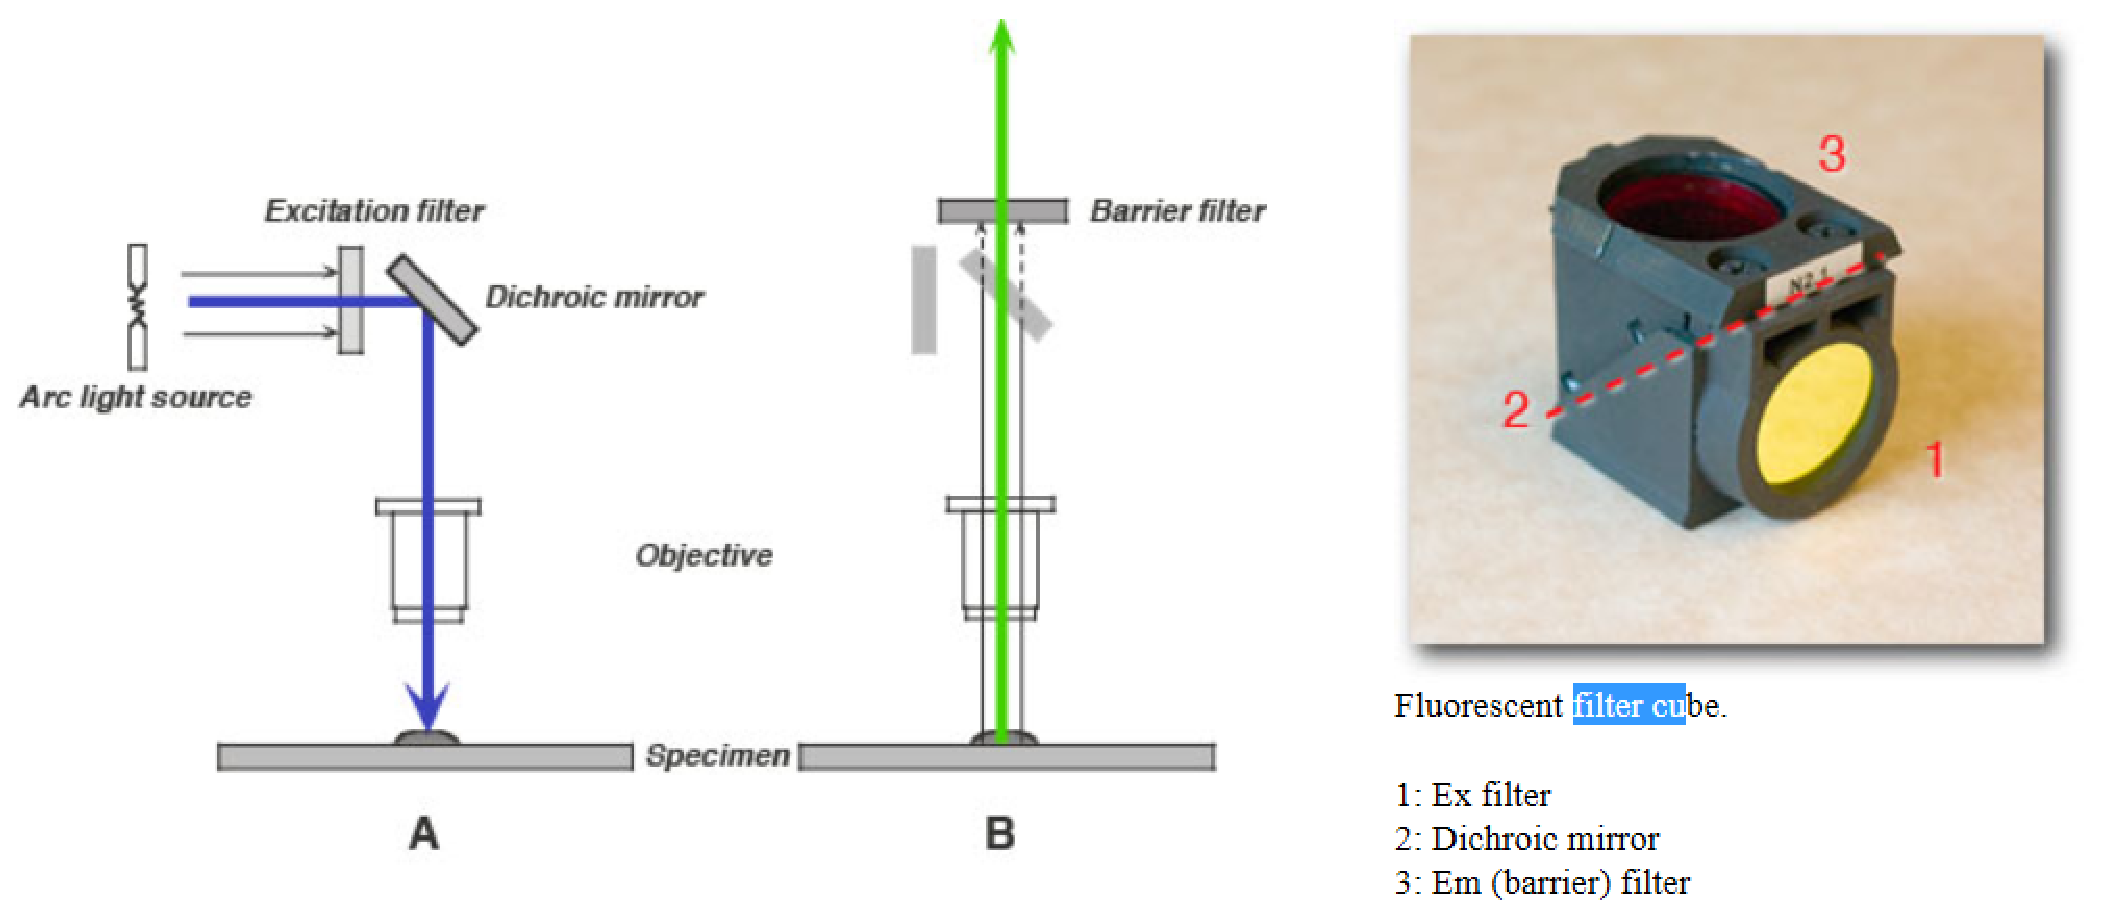
\includegraphics[height=5cm,
    angle=0]{./images/epifluorescence-microscope.eps}}
  \centerline{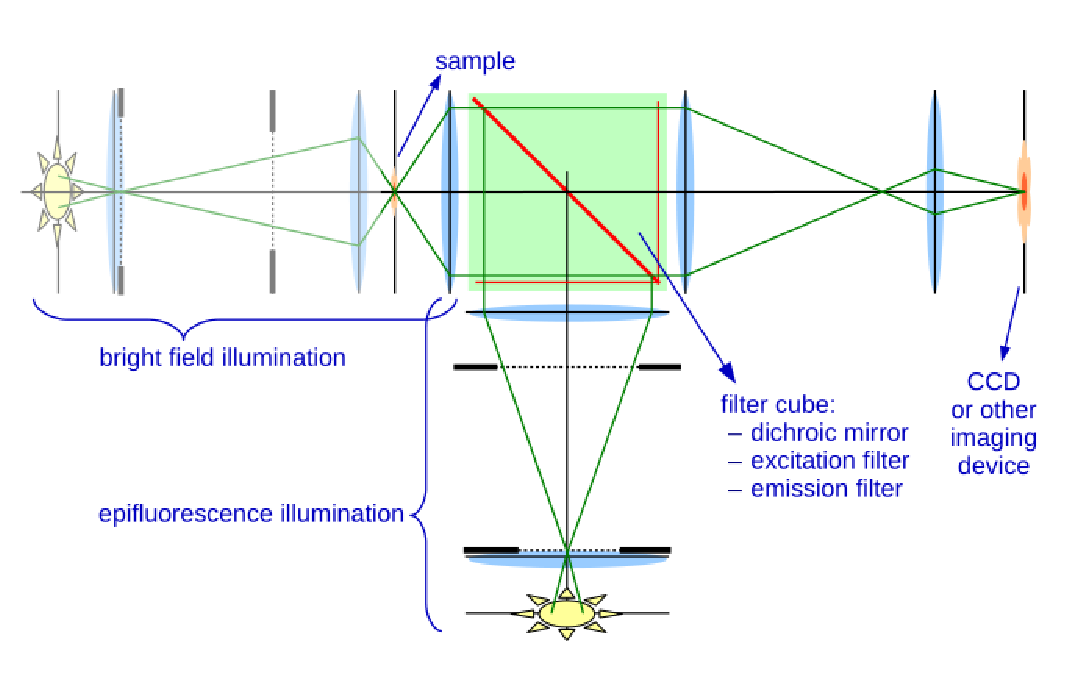
\includegraphics[height=5cm,
    angle=0]{./images/widefield_microscope.eps}}
  \caption{(A) Fluorescence cube; (B) How wide-field microscope works}
  \label{fig:widefield_micro}
\end{figure}

The weakness of wide-field epilfuorescence (Sect.\ref{sec:widefield_microscopy})
is that it has strong out-of-focus signal which limits the resolution of the
microscope, especially when making 3D visualization. The reason is that when the
light propagates through a distance larger than the wavelength of the emitted
light (i.e. wide-field or {\it far-field}); early solution was near-field
scanning optical microscopy (NSOM) to achieve high spatial resolution, giving
resolution 20-50nm. The short range of near-field is tens of nanometer make the
device limit to imaging near-surface features only.

Confocal microscopy (Sect.\ref{sec:confocal_imaging}) can filter
out out-of-focus light, by illuminating a single point at a time, giving
resolution 200-250nm. The limit of confocal microscopy is the resolution set by
diffraction limit. This becomes an issue when imaging subcellular structures
whose size is near or below the diffraction limit ($< 200$nm). 

The next far-field imaging technology is multiphoton microscopy
(Sect.\ref{sec:multi-photon_micro}).



\subsection{Laser-scaning Confocal microscopy}
\label{sec:confocal_imaging}

In laser-scanning confocal microscopy (LSCM) or just confocal microscopy, the
light source is laser. The laser light can focus on a small area/volume on the
focal plane (the specimens, or fluorescence) by the {\bf objective lens}. The
light from the laser triggered the reflected light (emitted energy) from the
specimen, and being recollected by the objective lens
\footnote{\url{http://www.bristol.ac.uk/synaptic/research/techniques/confocal.html}}.
As a result, a confocal microscope can generate high quality image (avoiding
blurring) by excluding most of the light coming from specimen that is not from
the microscope's focal plane. See:
\url{http://www.olympusconfocal.com/java/confocalvswidefield/}.
\begin{enumerate}
  \item adjusting aperture size: the larger, the more detail is captured, thus
  giving more noise.
  \item optical sections: capture the image at different Z-depth of a thick
  specimens, e.g. a cell, by adjusting the Z-axis position.
  \item scan-line speed: can also affect the result (the faster the speed, the
  lesser information can be capture as it need to stay long enough to have
  enough count rate per pixel).
  \item color map: can be changed by adjusting intensities of three different
  color channel (R, G, B).
\end{enumerate}
 
The laser beam scan the specimen from left to right and is rapidly transported
back to the start point in a process called {\bf flyback}. The size of the image
is typically 512x512, Fig.\ref{fig:LSCM_spot2image}, which can be built up in 1
second. The dwell-time for the laser at each point is typically 3.8$\mus$. An
optical section of 0.5-1.5$\mum$ through flourescent specimens up to 100nm
thick, non-invasively. \textcolor{red}{It has better lateral and axial
resolution than wide-field. It can do 3D (XYZ) or 4D (XYZt)-live cell imaging
with optical sectioning.}

\begin{figure}[hbt]
%   \centerline{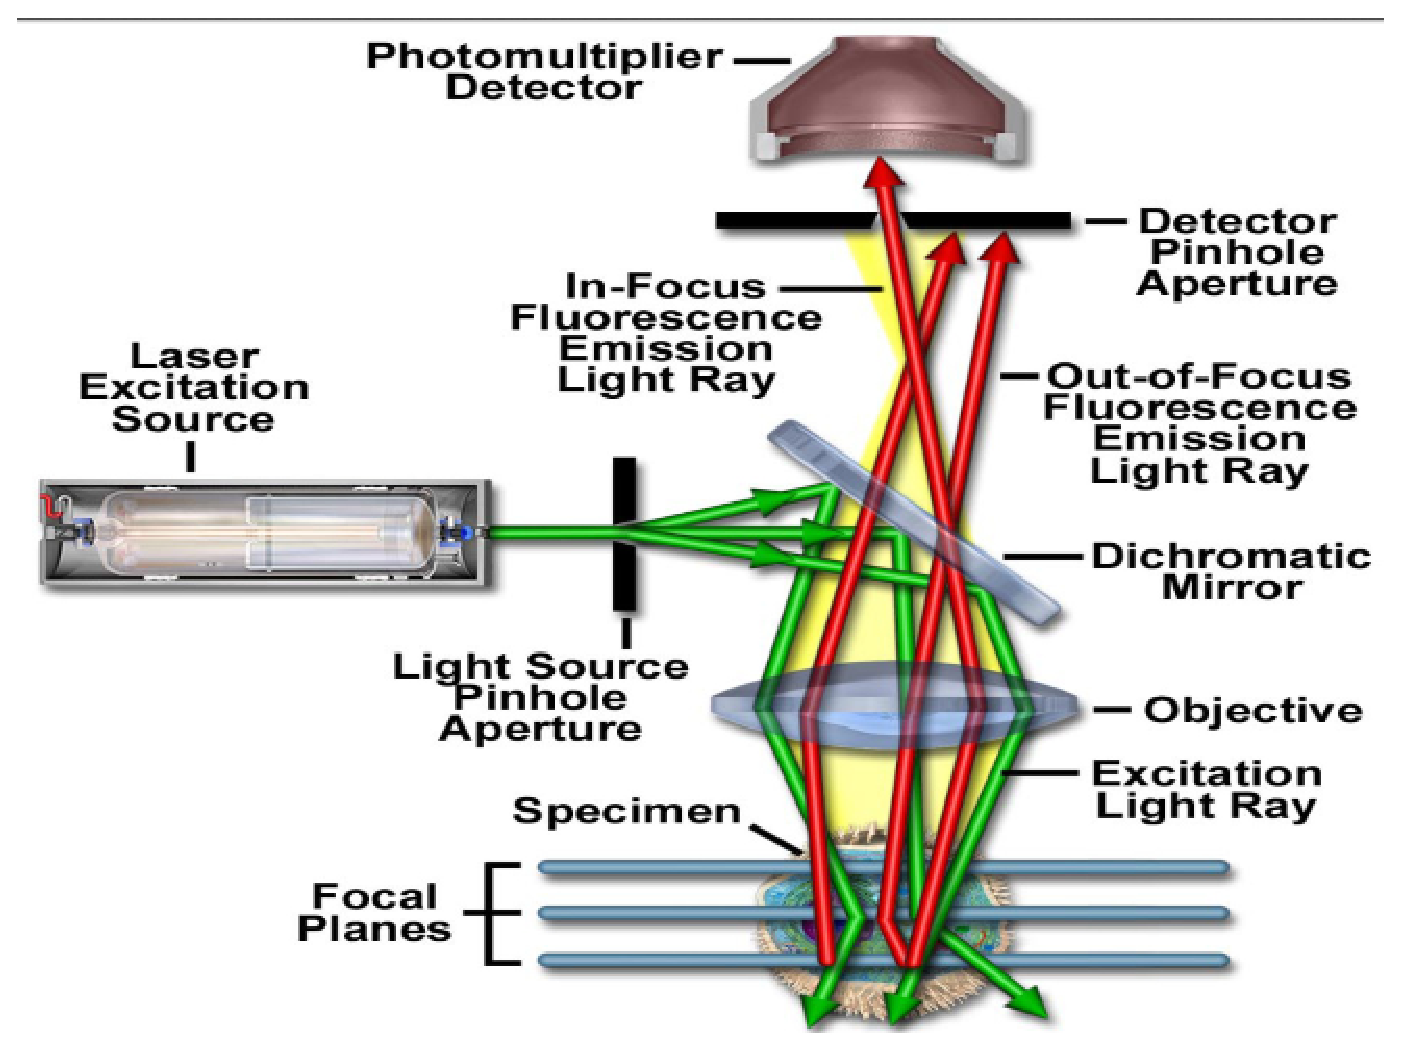
\includegraphics[height=4cm,
%     angle=0]{./images/LSCM_infocuslight.eps}}
  \centerline{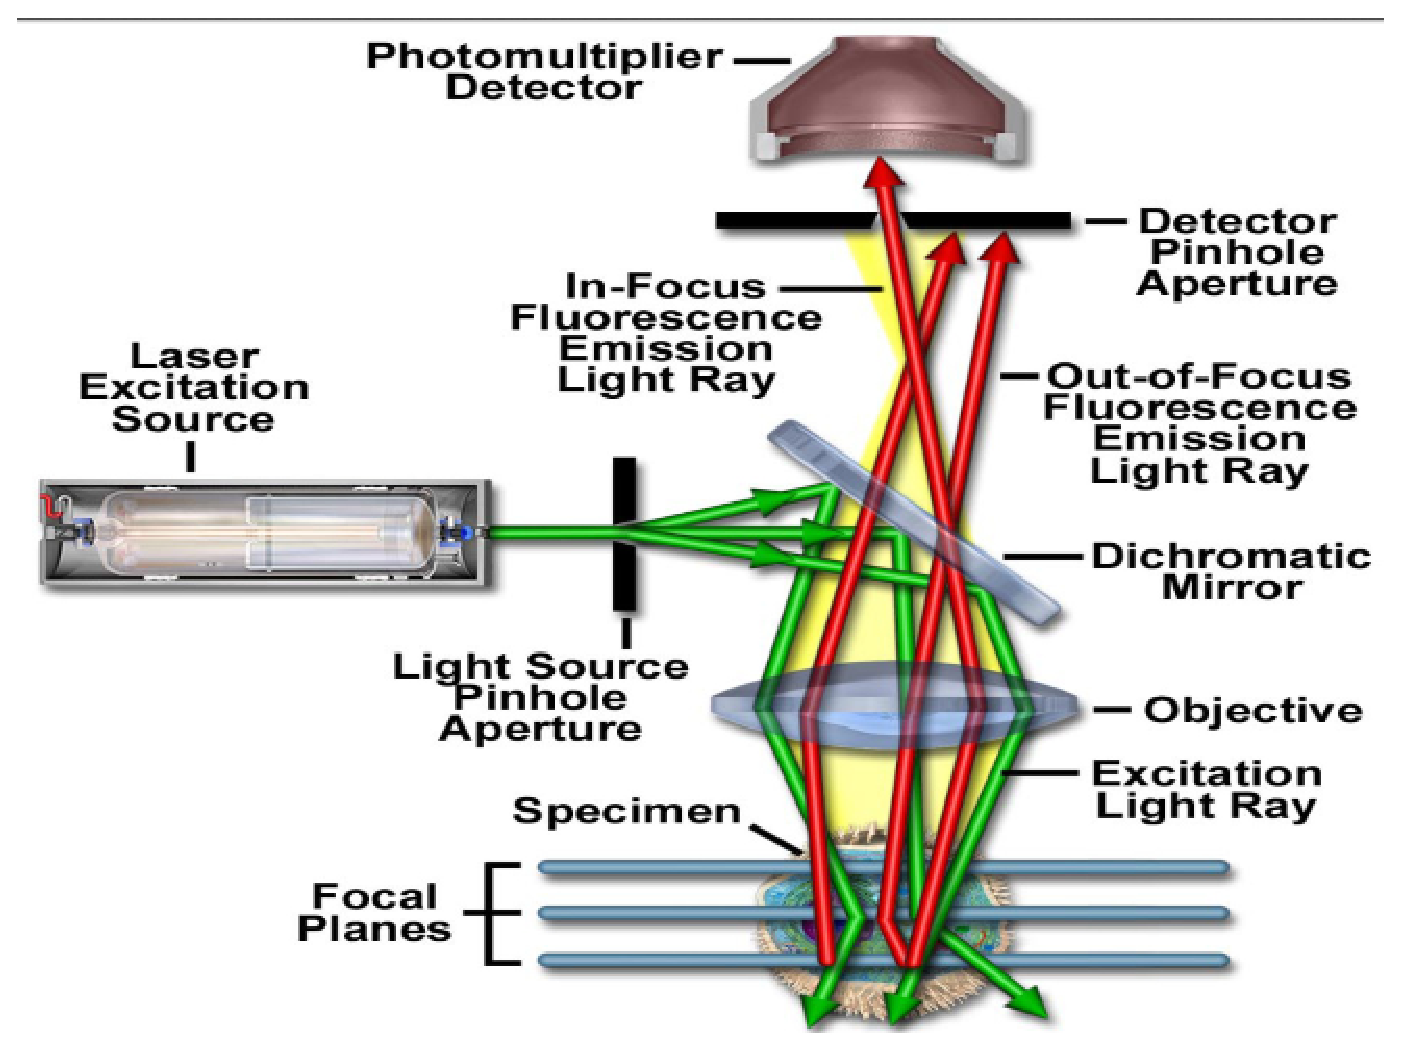
\includegraphics[height=5cm,
    angle=0]{./images/LSCM_infocuslight.eps} 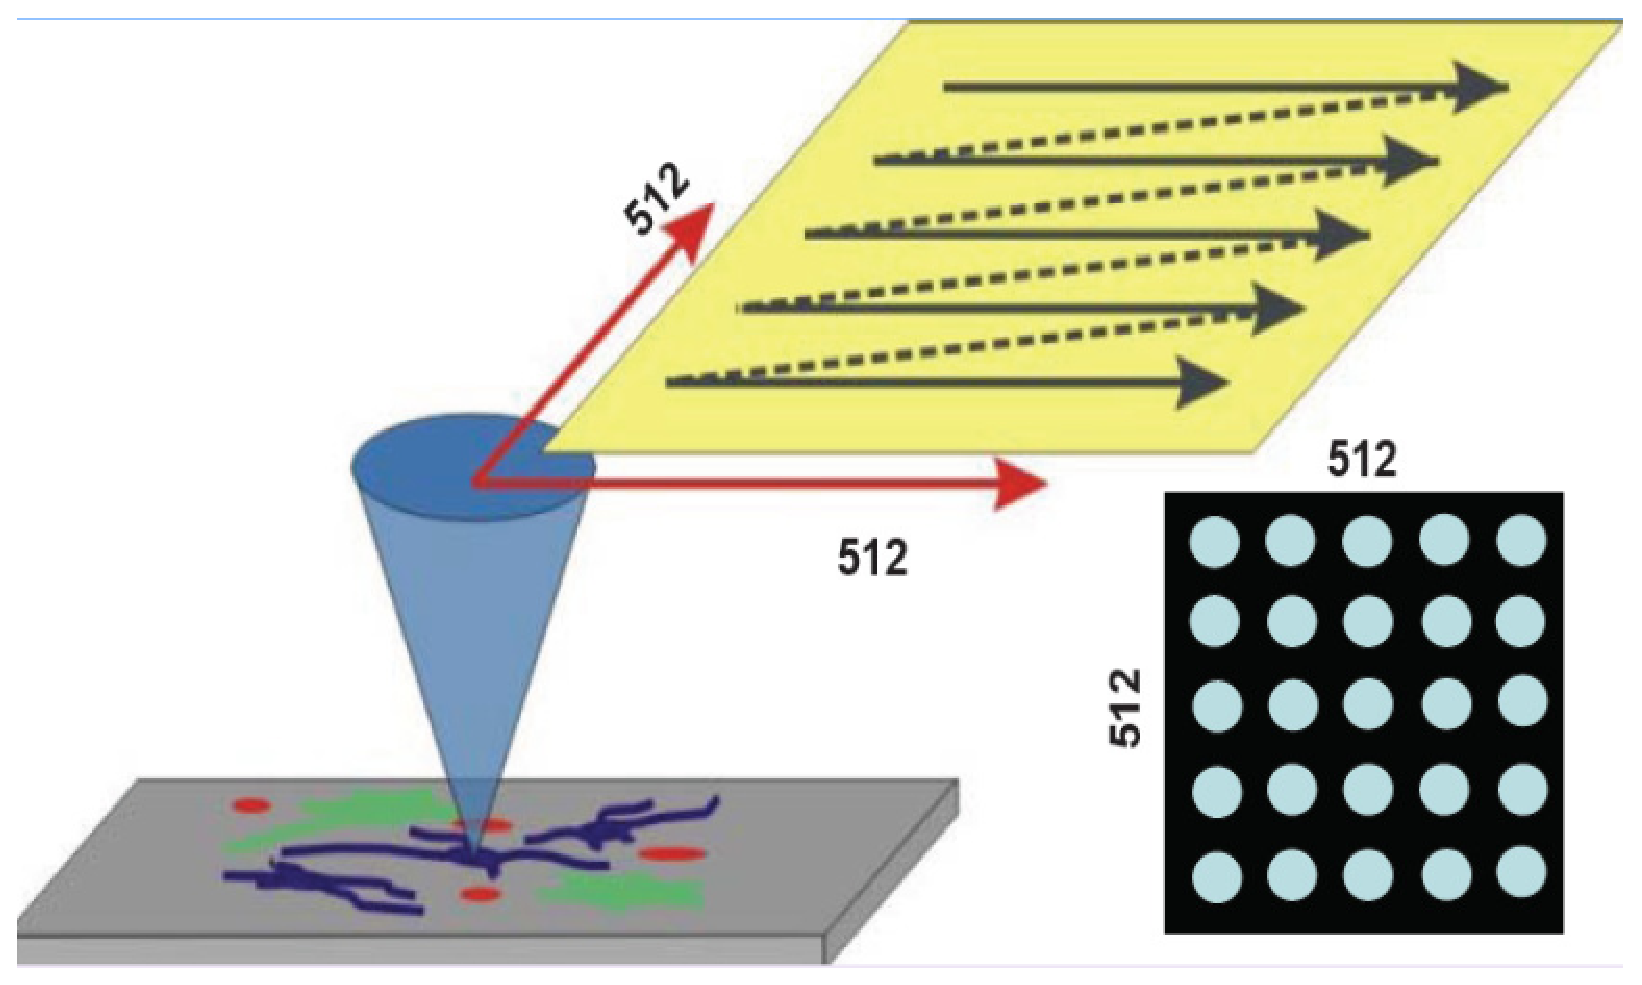
\includegraphics[height=3cm,
    angle=0]{./images/LSCM_spot2image.eps}}
  \caption{(A) Only in-focus exciting and emitted light are detected; (B) How 2D
  line-scanning image are generated}
  \label{fig:LSCM_spot2image}
\end{figure}


The fundamental weakness of confocal microscopy is that the strong laser beam
also excite the specimen above and below the focal plane. The excitation light
is scattered as it passes through tissue, solutions bathing the sample, glass
coverslips. The pinhole is placed in front of the photo-multiplier tube (PMT) to
block the passage of this out-of-focus light into the PMT. So, only light comes
from the near focal plane of the objective lens of the microscope. It can also
produce the image taken across the area of the sample, giving a slice through
the object and surrounding material, known as optical slicing that allows us to
see inside the object of interest. To generate 3D image, different slicing
images are taken at different depths. The images are stacked on top of one
another in the correct order to generate a single image of the object.

\begin{framed}
The early device developed by Minsky can generate 1 image per every 10 sec. New
devices have been improved in speed, image quality.
\end{framed}

Confocal fluorescence microscopy consists of multiple laser excitation sources,
a scan head with electronic and optical components, electronic detector (e.g.
photomultipliers), and a computer for acquisition, processing, analysis, and
display of images. The photomultiplier, using 10-12 bits, is capable of
displaying 1024 to 4096 gray levels. However, the photomultiplier being used in
commercial confocal fluorescence microscopy has the dynamic range limited to
8-bit (256 gray levels) which is adequate to handle number of photons per pixel. 

 \begin{figure}[hbt]
  \centerline{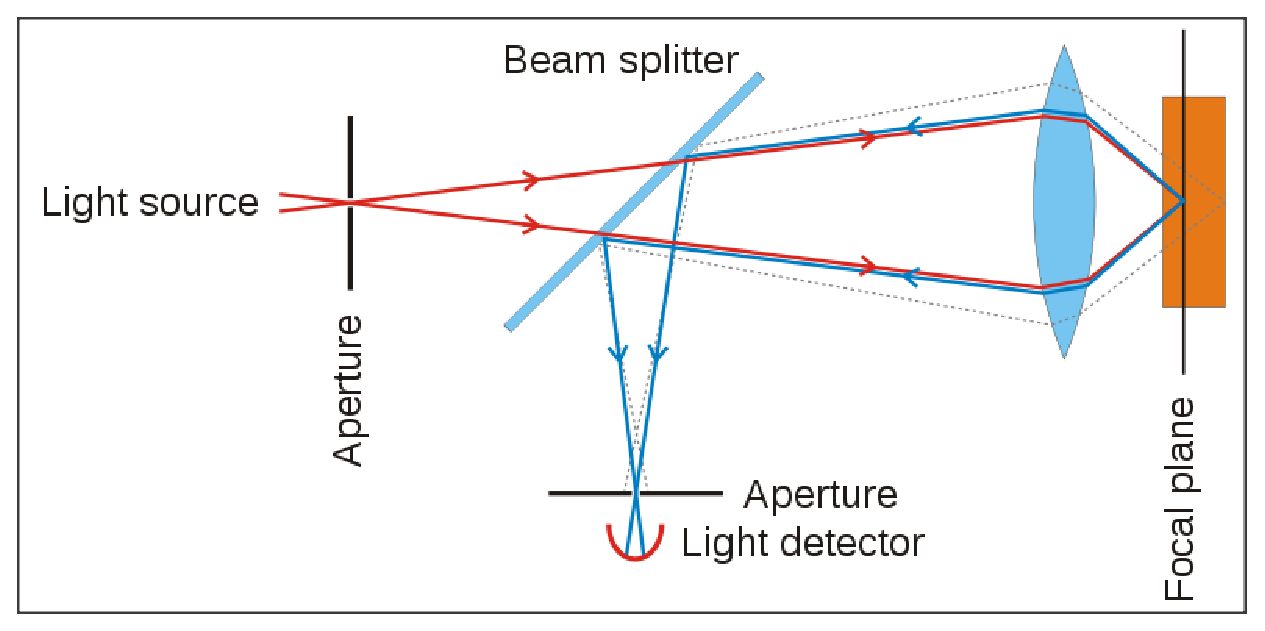
\includegraphics[height=5cm,
    angle=0]{./images/confocal_microscope.eps}}
\caption{Principle of confocal microscope}
\label{fig:confocal_microscope}
\end{figure}


The visualization of the detector is done on a personal computer, which builds
up the image one pixel at a time. A 512-by-512 pixel image is generated at a
frame rate 0.1-30 Hz. Confocal laser scanning microscopy (CLSM) allows
obtaining high-resolution optical images from a selected depth (z-resolution or
depth) via the process {\bf optical sectioning}. A conventional microscope can
``sees'' in depth as far as the light can penetrate. However, for CLSM, only
images at one depth level can be captured at a time.


The size of the small volume $(\delta x, \delta y, \delta z)$, its location
(x,y,z), and the number of photons that pass into $n_1$ and out of $n_2$ of the
focal plane. If the average result is $n$ photons/measurement. Then, based on
Poisson distribution, the variance is also the mean $\sqrt{n}$, 63\% of the
measurements will fall into $n\pm \sqrt{n}$. Such measurement is said to have
10\% statistics. So to increase the accuracy to 1\%, it needs $(100)^2=10,000$
photons. For a 1mW laser beam that can produce $10^{15}$ photons/sec, this can
become a detected signal of only 10-100 photons/pixel. 

High-end confocal microscope system can have several photomultipliers, allowing
simultaneously measurement different fluophores in multiply labeled specimens.
We can combine fluorescence contrast with phase contrast and differential
interference contrast (DIC). Modern systems with 3-5 lasers can be controlled by
high-speed acousto-optic tunable filters (AOTF), which allows very precise
regulation of wavelength and excitation intensity. This allows the development
of new techniques: FRAP (Sect.\ref{sec:FRAP}), FLIP (Sect.\ref{sec:FLIP}) .

% \subsection{Fluorescence confocal microscope}
% \label{sec:fluo_microscope}	

The fluorescent substance is typically fluorophore. The light that we detected
is emitted by the fluorophore that attach to the sample we want to measure.
Depending on the ratio of binding, e.g. linear binding where one Fluo bind to
one calcium, we can induce the level of calcium based on level of CaF. There is
a filter to filter out the other wavelength to keep only the wavelength emitted
from the calcium-bound fluorophore.

Two avalance photodiodes (APD) as fluorescence detector to overcome the limited
{\it photon counting rate} of a single APD ($\sim 5$MHz). Photon-counting rate
(a digitalized method) offers a better accuracy and improved SNR at low levels
than analog methods. Photon-counting can be done with APD or PMT
(Photomultiplier tube). APD is better than PMT in measuring low levels of light,
as it has higher quantum efficiency (QE) than PMT at the wavelength of interest.
PMT is, on the other hand, more efficient when using low background fluorescent
(F0). 

Typically, in a confocal system, there's a system's {\it dead time} during
which the system is insensitive to incoming photon. So, we may need a correction
factor. Yet, we should not overuse correction factor as it may decrease SNR,
i.e. increase uncertainty. In two-photon system, dead time of amplifier
discriminator (model 1181, EG\&G PARC) is 20ns, which is similar to two-APD
system. 

\begin{framed}
The pixel value is represented by the {\bf count rate}.
Correction factor should be kept as low as possible. \citep{wier2000} used a
two-photon microscope with dead time of $\sim 40\times 10^{-9}$ (sec), and the
correction factor is calcualted. Correction factor is 1.37 (for two-APD
dectors at a recorded coun rate of 10 MHz), and 2.0 (single APD).

The pixel duration should be long enough to have enough count rate per pixel.
E.g.: in single-APD system, count rate of 5 MHz can be measured accurately
with pixel duration 10.0$\mus$, not 1.0$\mus$. Then, with 10.0$\mus$, each pixel
contains, on average, 50 counts. The variance, at peak $\Ca$ sparks, is about
7.07, or 0.707 MHz, while with 1.0 $\mus$-pixel, the variance is 2.24 MHz. Here,
larger variance requires using larger correction factor. 

\end{framed}

The low level means $< 5$ counts/pixel or $0.5\times 10^6$ counts/sec, and this
count rate can be fit by Poisson distribution. At higher level, the
distributiono approaches normal (Gaussian).
\begin{verbatim}
SNR = mean/variance
\end{verbatim}
Count rates, even at the peak of $\Ca$ sparks, recorded with two-photon systems
are generally $< 2\times 10^6$ counts/sec. 


\citep{wier2000} developed a confocal component 9x more efficient than the
commercial confocal microscope (Fluo-4). The resolution of the confocal
microscope is 0.25$\mum$ laterally and 0.52$\mum$ axially. For two-photon
system, the resolution is 0.28$\mum$ and 0.82$\mum$. Also, cellular volume on
the order of $10^{-15}$ littre can be detected.

PSF of the x60 1.4-NA oil-immersion objective lens has lateral FWHM was
0.25$\mum$ and axial FWHM was 0.52$\mum$. The same lens, yet now in two-photon
system has 0.28$\mum$ and 0.82$\mum$. Here, pixel dimensions were 0.05$\mum$
laterally and 0.1$\mum$ vertically. 


In laser scanning confocal fluorescence microscope, the spatial resolution in
lateral direction is about $0.6\lambda/\sqrt{2}. NA$, and axial direction of
$1.4\eta\lambda. (NA)^2$, with NA is numerical aperture, $\lambda$ is the
excitation wavelength, $\eta$ is the medium refraction index (NOTE:
$NA=\eta\sin\theta$.

In wide-field microscopy
\begin{equation}
r_\text{lateral} = 1.22\lambda / (2. NA)= 0.6\lambda/NA   
\end{equation}
In confocal microscope
\begin{equation}
r_\text{lateral} = 0.4\lambda/NA
\end{equation}
The depth of the field
\begin{equation}
r_\text{axial} = 1.4\lambda .\eta/(NA)^2
\end{equation}

\subsection{Multi-photon (e.g. Two-photon) laser-scanning confocal microscopy}
\label{sec:multi-photon_micro}

Multi-photon system use two- or three-photon absorption. Its use in calcium
imaging in nervous system started in 1995 (Yuste and Denk, 1995).

\subsection{-- Two-photon confocal microscope}
\label{sec:two-photon-confocal-imaging}

The introduction of two-photon microscopy by Winfried Denk and colleagues (Denk
et al., 1990) is a major breakthrough \citep{denk1990}.

Two-photon confocal microscopy addresses a fundamental drawback of
(single-photon) confocal laser scanning microscopy, i.e. avoiding out-of-focus
excitation and can image deeper into a specimen (than $\approx 400 \mum$).
In one-photon microscopy, the beam can excite the specimen above and below the
focal plane which cause more noise, Fig.\ref{fig:confocal_micro}. In two-photon
microscopy, the emitted light is only from the focal volume.

To avoid using high-energy light beam, but still can generate high enough
energy, multiple low energy incident light are combined (to the same point in
space in a sufficiently short time that the energy effectively is summed and so
acts as a higher energy single photon \citep{semwogerere2005}) to generate high
energy fluorescence.

This can avoid out-of-focus occur caused by single-photon excitation which can
happen at low-laser intensity, but two-photon excitation require high laser
intensity (Sect.\ref{sec:multi-photon_micro}).
Importantly, no pinhole is required in multiphoton LSCM.




\begin{figure}[hbt]
  \centerline{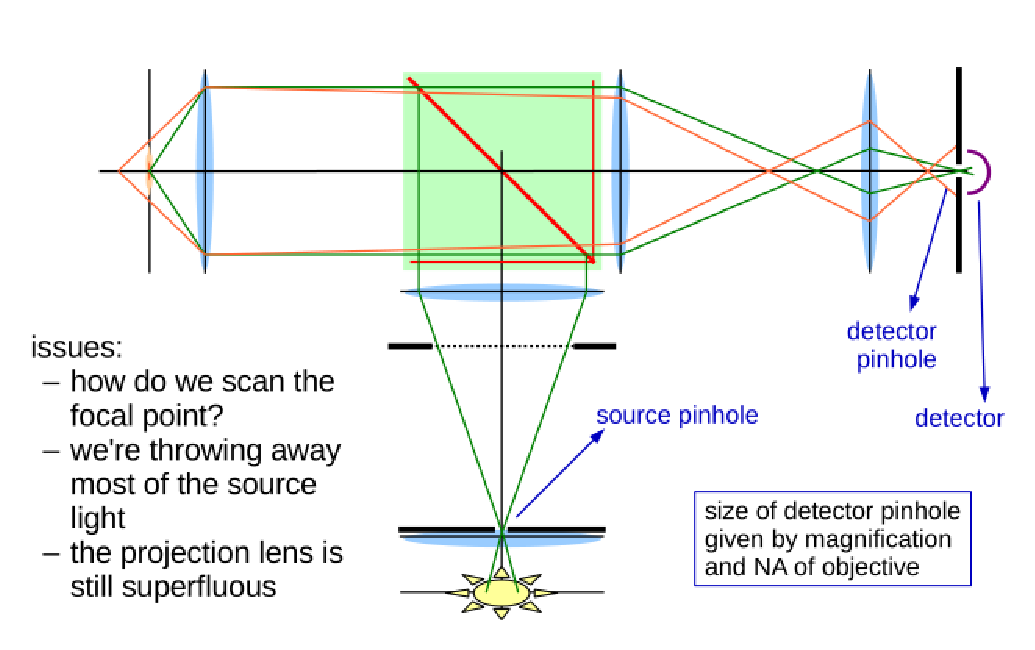
\includegraphics[height=5cm,
    angle=0]{./images/confocal_microscope3.eps}}
    \centerline{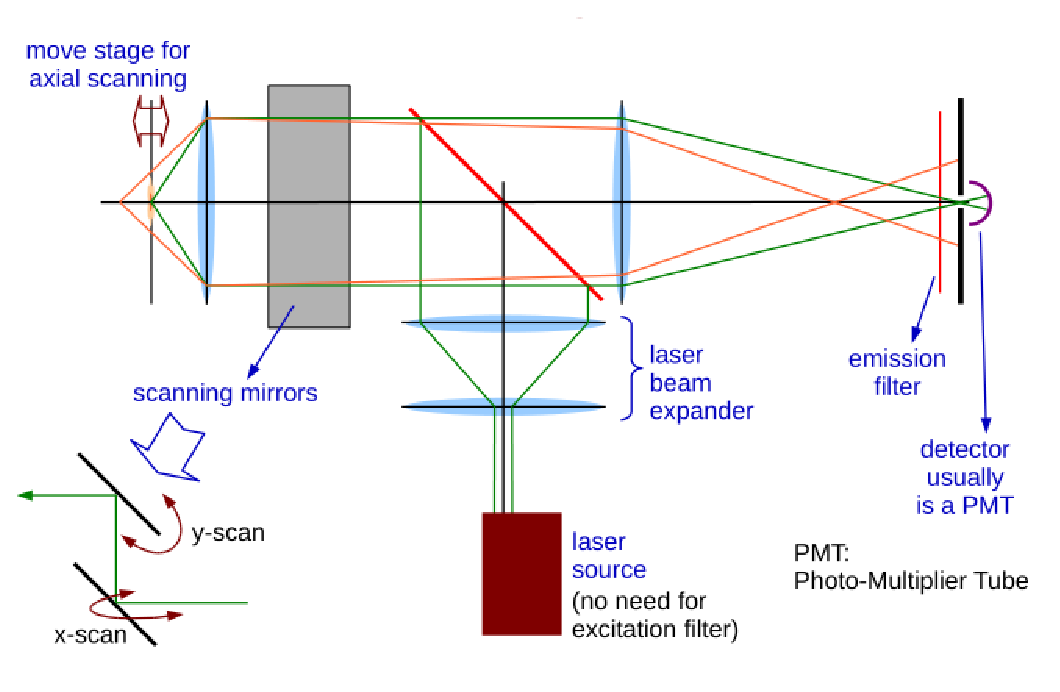
\includegraphics[height=5cm,
    angle=0]{./images/confocal_microscope4.eps}}
  \caption{How confocal microscope works (A) capture 2D; (B) capture 3D}
  \label{fig:confocal_micro}
\end{figure}

The weakness of confocal microscope is scanning one dot at a time which is slow.
The solution is using multi-focal scanning confocal or spinning disk
confocal (i.e. both helps scanning multiple dots at a time) or line-scanning
confocal (scan one line at once)
(Sect.\ref{sec:multipoint_scanning_microscopy}).

\subsection{-- Multi-photon excitation}

Energy are released/absorb in quantum forms known as {\bf photon}. One photon
energy $\propto 1\lambda$. So 1photon = $\lambda$, 2photons = $2\lambda$,
3photons = $3\lambda$. An electron increases to a new
energy level when abdorbs photon, and relax when it emits photon. 

Photon absorption probability is propotional to the square of photon density
(i.e. nonlinear). The probability for two-photon absorption is very low at
moderate light intensities (e.g. in bright sunlight, the probability is once
every 10 million years \citep{denk1997}). Also, fluorescence excitation occur
only at focal point, so no need to filter out-of-focus light.
\textcolor{red}{Less scattering means it allow deeper penetration and higher
axial resolution}, in a cost of lower x-y resolution.
Without using pinhole, scattered fluorescent light still can be collected.

The drawback of this method is that huge photon density is required (using
pulsed laser) to generate high enough light intensity at the focal point and
thus it's more expensive.
\begin{itemize}
  \item femto-second pulsed lasers: Ti:Sapphire (titanium-sapphire) laser
\end{itemize}

\subsection{-- Two-photon laser scanning microscope (2PLSM)}

Two-photon laser scanning microscope (TPLSM) uses two infrared photons produced
by mode-locked pulsed laser 

\subsection{Multipoint scanning confocal microscopy (spinning disc)}
\label{sec:multipoint_scanning_microscopy}

Detectors for multipoint scanners like spinning-disk confocals can collect
spatial information. Many pinholes are put in a Nipkow disc.


Here, multiple points are excited at once and it's critical
to discriminate photons coming from one point in the image from those photons
generated in a different location. For this reason, cooled CCDs are the choice
for detectors, rather than PMT \citep{jerome2011dic}. A CCD has a matrix of
photodiodes sensors capable of sensing photons. The light failing on each sensor
creates an electric charge proportional to the light intensity at that location.
The charge is then read and converted into a voltage. Some examples of spinning
microscopes are given in Fig.\ref{fig:spinning_microscope}. 

\begin{figure}[hbt]
  \centerline{
%   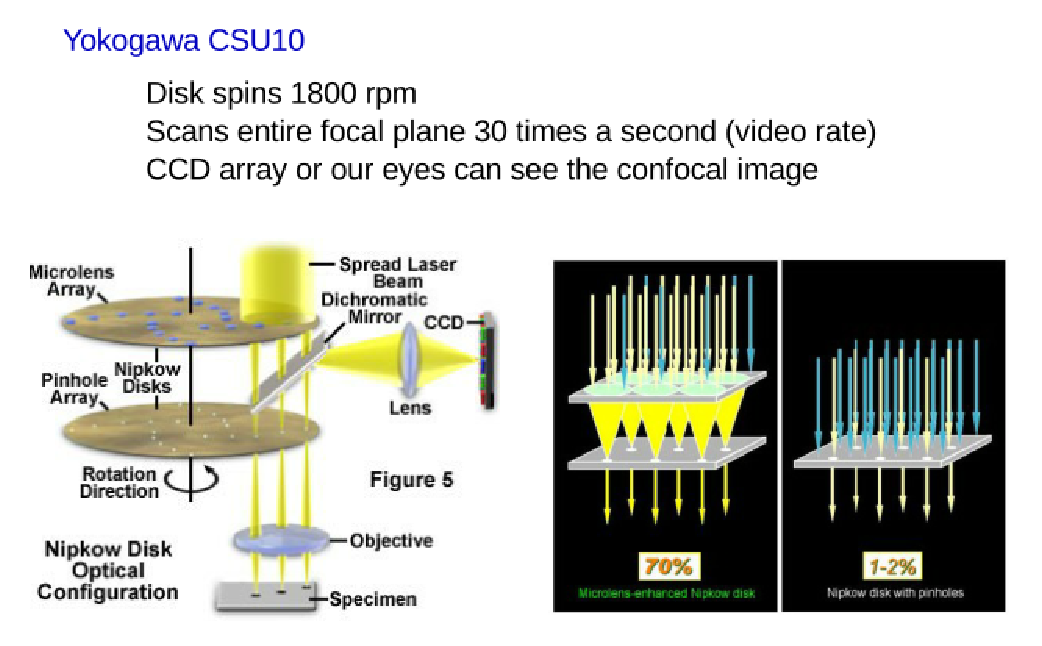
\includegraphics[height=5cm,
%     angle=0]{./images/spinningdisk_microscope.eps}}
    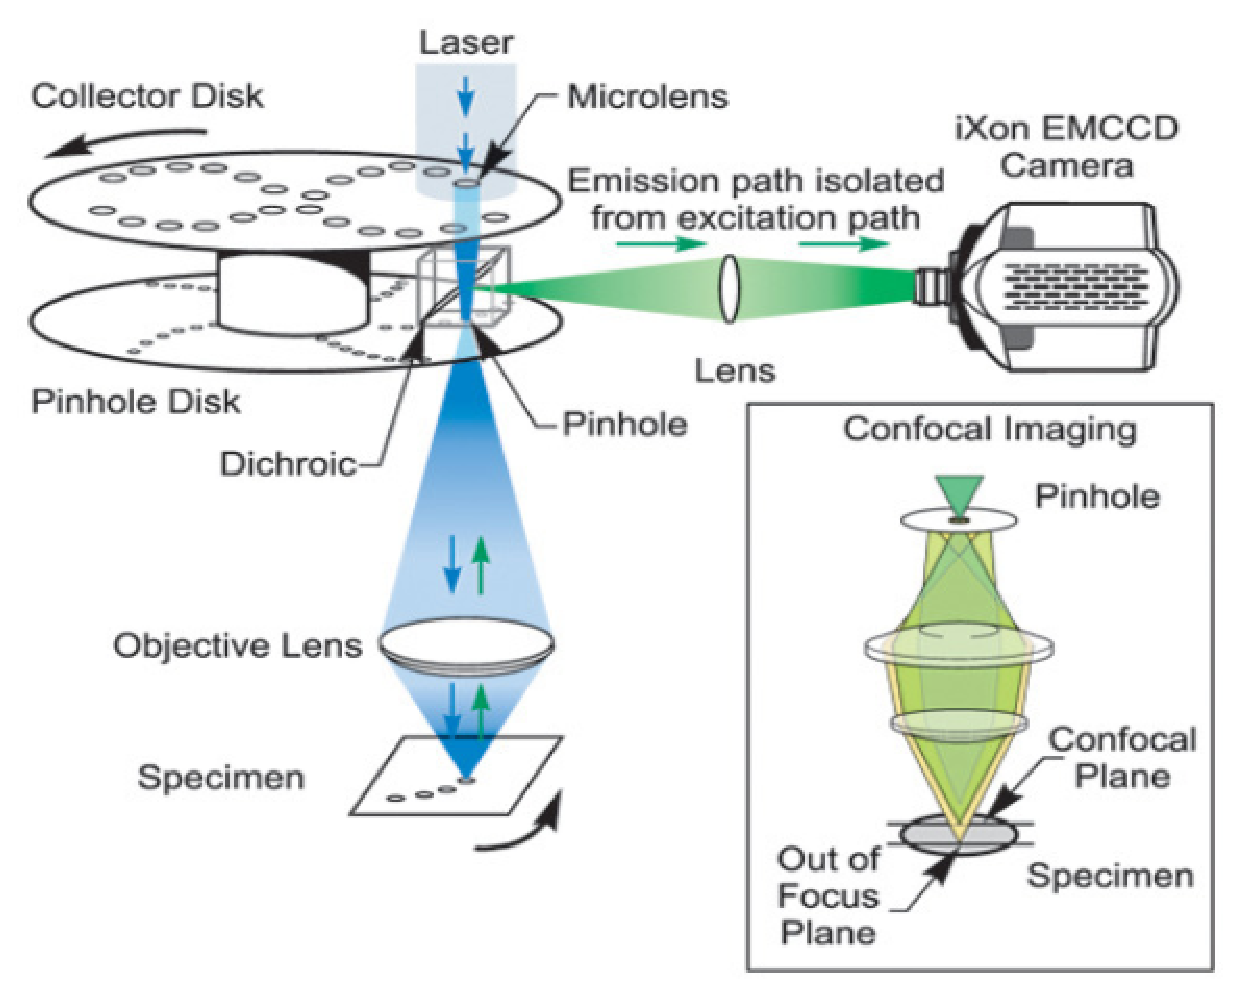
\includegraphics[height=5cm,
    angle=0]{./images/LSCM_spinningdisc.eps}}
      \centerline{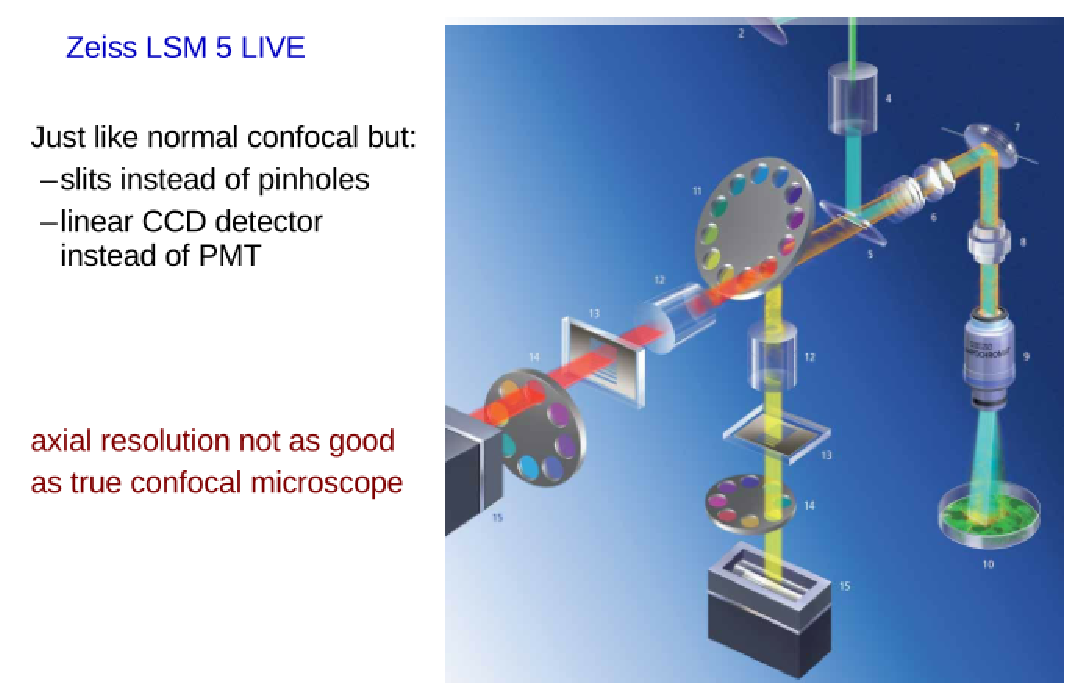
\includegraphics[height=5cm,
    angle=0]{./images/spinningdisk_microscope2.eps}}    
  \caption{Spinning microscope (A) Yokogawa CSU10, (B) Zeiss LSM 5 Live (with
  slits instead of pinholes)}
  \label{fig:spinning_microscope}
\end{figure}

As CCD is not as sensitive as PMT, and the time to collect an image and transfer
to the computer memory is slower than that of PMTs, the axial resolution is not
as good as true confocal microscope. Unlike PMTs, the CCD photodiodes do have a
physical size. A popular sensor size if 6.45$\mum$ in each dimension
\begin{enumerate}
  \item A lense with N.A.=1.3 (pretty standard for water immersion lens) with
  size little less than 0.2$\mum$ in diameter. If the magnifying power is 63x,
  then the smallest resolved objects (which is defined as the Airy
  disk diameter $\approx 0.2 \mum$) is projected onto the chip of size
  12.6$\mum$ which is about 2x the sensor size. 
\end{enumerate}
The smallest resolved object here is roughtly twice the size of
the sensor. This is important because of a key concept in sampling statistics
called Nyquist-Shannon theorem (or Nyquist theorem or Nyquist criterion) which
states that the analog signal can be perfectly reproduced if the
smallest element (i.e. the elements of smallest frequency, as the analog signal
is digitally represented as the sum of a number of sinual
signals of different frequencies) is sampled at least twice. In the case of
image reconstruction, Nyquist-Shannon tells us that the sampling probe must have
the diameter of half the size of the object in both X and Y-directions. In
practice, the sampling interval is often set to 2.3x smaller than the smallest
element.

The array size of a CCD camera for scientific studies are in the range of
1000x1000 pixels to 5000x5000 pixels, with an individual sensor of size
6.45$\mum$. So, a 1000x1000 array of sensors can capture an area of size
6450$\mum$x6450$\mum$. With 63x lens, the captured image contains the
information from an area of size 102$\mum$ x 102$\mum$ (as 6450/63=102).
NOTE: Larger cameras can capture a larger area, yet in the expense of a slower
readout rates.


For multi-focal, they used micro lens array lined up with pinhole
array, Fig.\ref{fig:multifocal_microscope}.

\begin{figure}[hbt]
  \centerline{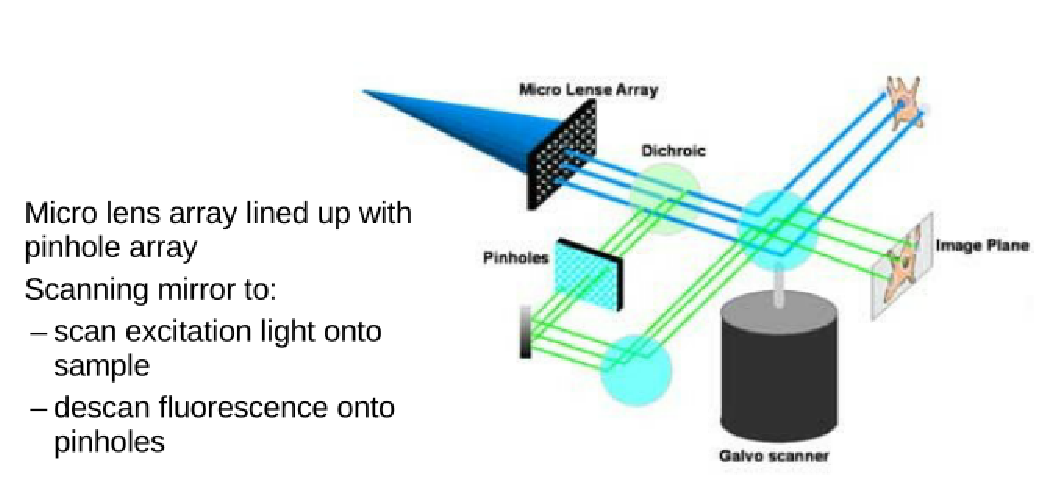
\includegraphics[height=5cm,
    angle=0]{./images/multifocal_microscope.eps}}
  \caption{Multifocal microscope}
  \label{fig:multifocal_microscope}
\end{figure}

\subsection{4Pi microscope (better for 3D images)}

The diffraction limit given by $\NA = \eta \sin\theta$. To increase the
resolution, the two approaches are
\begin{enumerate}
  \item increase $\eta$ (impractical)
  \item increase aperture angle $\theta$ (limited to $\theta \approx 74^\circ$,
  but can be increased???). $4\pi$ solid angle is full sphere by using 2
  opposing high-NA objectives to coherently illuminate and detect the same
  point of the fluorescence speciment.
\end{enumerate}
Single-photon 4Pi microscope provides 4x narrower PSF in lateral, but highly
enlarged axial sidelobes. So it's doesn't produce better 2D images than
other confocal microscope. However, two-photon 4Pi microscope can produce better
3D images \citep{blanca2001}.

\subsection{STED (Stimulated Emission Depletion) microscope}
\label{sec:STED}

Fig.\ref{fig:STED_microscope} show how it's better than confocal microscope.
STED can create sub-diffraction limit resolution by altering the effective PSF
of the excitation laser beam by using a second laser that suppresses
fluorescence emission from fluorophores located away from the center of the
excitation. This also narrow down the PSF and ultimately increase the resolution
beyond diffraction limit. STED microscopy can deliever 20nm (or better) lateral
resolution and 40-50 nm axial resolution.

\begin{figure}[hbt]
  \centerline{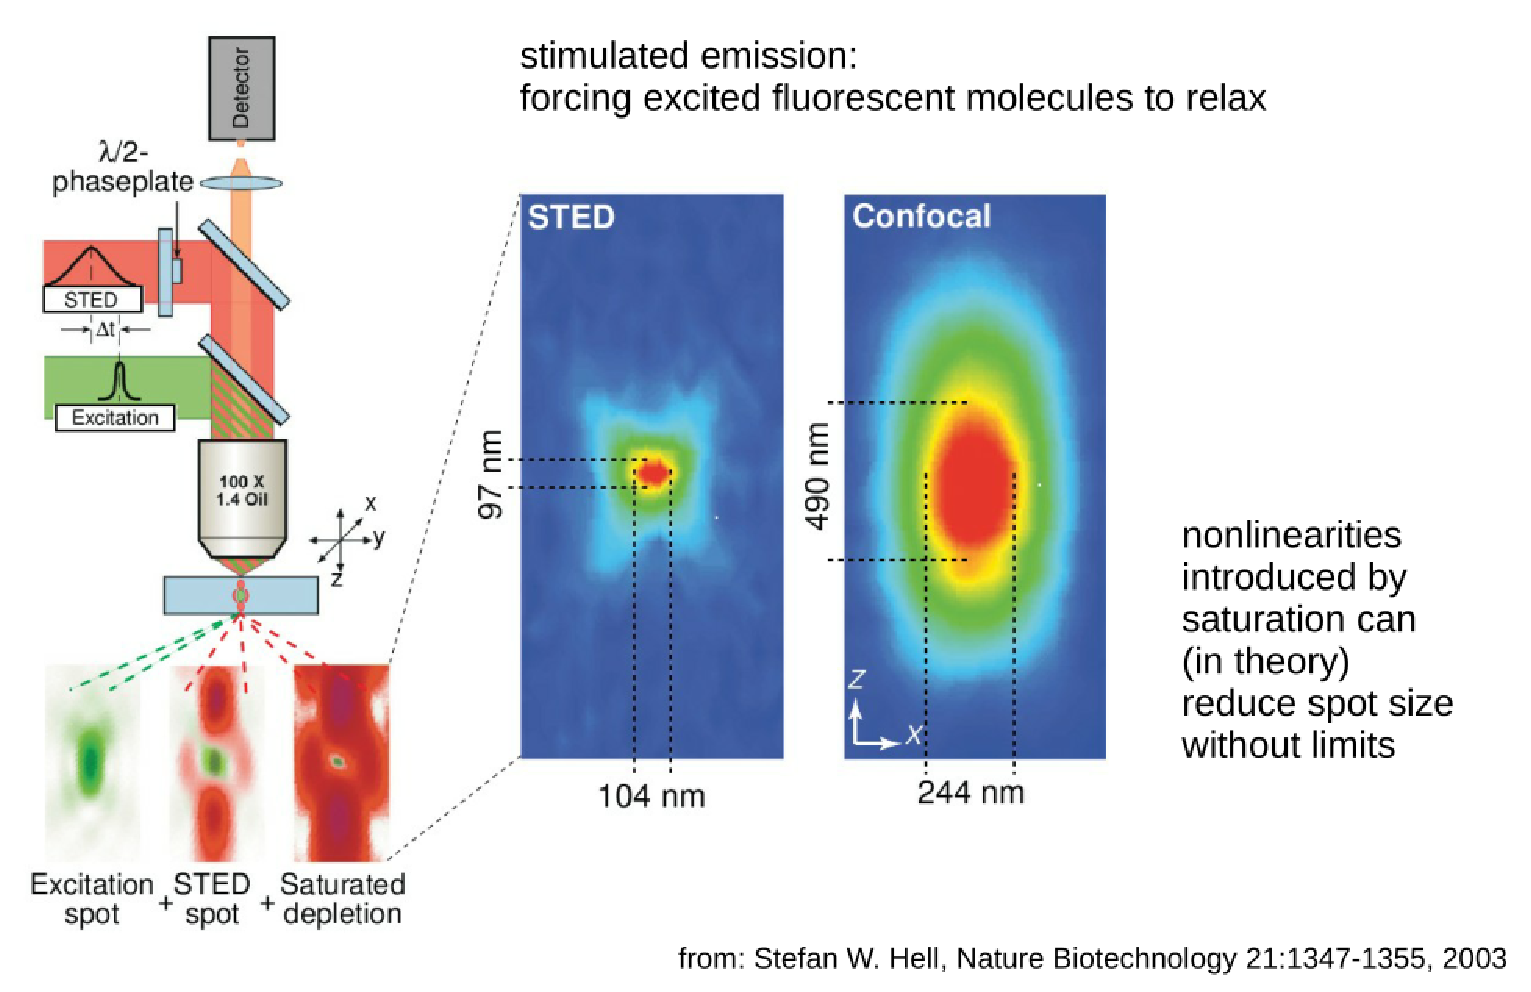
\includegraphics[height=5cm,
    angle=0]{./images/STED_microscope.eps}}
  \caption{STED microscope}
  \label{fig:STED_microscope}
\end{figure}

To assess the resolution, images of sub-resolution (20nm) crimson beads were
collected. Images of three aligned beads were averaged, and the central line of
the image was fitted with the Gaussian function to assess the lateral
resolution. The size of 30nm translate to 1-2 RyR tetramers in the focal
plane. To detect RyR, fluorescence Atto 647N is used to label RyR. As the
fluorescence level is lower, deconvolution was required to improve the
signal-noise, and further improvement of image resolution to allow automatic
image thresholding.

The suppression is achieved when an excited-state fluorophore encounters a
photon that matches the energy difference between the ground and excited-state.
These fluorophore return to the ground state through stimulates emission before
spontaneous fluorescence emission can occur. This process can effectively
depletes selected regions near the focal point of excited fluorophores. See:
\url{http://zeiss-campus.magnet.fsu.edu/tutorials/superresolution/stedfundamentals/}

\subsection{Photo-Activated Localization Microscopy (PALM)}
\label{sec:PALM}

Recent advancements allow using genetically-encoded fluorescent proteins that
act as an endogenous labels to enable virtually imaging any peptide or protein.
This allows precise detection the location of single protein molecule.


The goal is to minimize background noise and maximize photon output 



\subsection{Stochastic Optical Reconstruction Microscopy (STORM)}

\subsection{Total Internal Reflection Fluorescence (TIRF)}

TIRF requires very hig NA lens (1.4 or higher).

\section{Advanced fluorescence techniques}

There are specialized applications of confocal microscopy.

\subsection{FRAP (photobleaching)}
\label{sec:FRAP}

FRAP  = (fluorescence recover after photobeaching). FRAP is used to study the
diffusion rate of fluorescent-tagged protein. The term {\bf caged} refer to
unactivated fluorescence molecules bound to photsensitive species. When it is
activated by intense illumination that free them from the caging compounds

\subsection{FRET}
\label{sec:FRET}

FRET (Forster (or Fluorescent) resonant energy transfer) is the technique that
allows us to identify the colocalization of two specimens (e.g. protein-protein
interaction) within intact cells by  measuring changes in fluorescence resonance
energy transfer (FRET) between the cyan (CFP) and yellow (YFP) variants of green
fluorescent protein (GFP).
So, it's used for protein interaction studies \citep{karpova2006}
% https://www.ncbi.nlm.nih.gov/pubmed/18770833
YFP-tagged protein (the FRET "acceptor") is photobleached at a cellular site of
interest, and then the intensity of the CFP-tagged protein (the FRET "donor") at
that same site is measured. In principle, FRET is detected when the CFP
intensity increases after the photobleaching of YFP.

FRET can be conveniently measured as the ratio of donor (480 nm) over acceptor
emission (545 nm) intensities when cells are excited at the donor excitation
wavelength (440 nm). Changes in fluorescence ratio (480 nm/545 nm) are directly
correlated to changes in C and R subunit association.

Example: 
\begin{itemize}
  \item  SERCA-PLN FRET can tells us whether SERCA and PLN are bound to each
  other or not; where SERCA bound to Cerulean and PLN bound to YFP.
  
   \item 
\end{itemize}

Example: cAMP concentration detection with PKA phosphorylation
(Sect.\ref{sec:PKA}) using CFP- and YFP-tagged proteins
\begin{itemize}
  \item cAMP is detected using genetically encoded cAMP probe \citep{Zaccolo2002,
Nikolaev2006}, by fusing R and C subunits of PKA to CFP and YFP, respectively.
  
GOAL: to monitor PKA regulatory (R) and catalytic (C) subunit dissociation due
to a rise in the intracellular cAMP concentration leading to phosphorylation of
PKA. 
  
  \item At low [cAMP], then GFP-tagged PKA is inactive state
  (CFP-R$_2$C$_2$-YFP): FRET signal is at maximal
  
  \item At high [cAMP], cAMP binds to R-subunit (CFP) and inducing a
  conformational change that releases active C; CFP and YFP diffuse apart and
  FRET is abolished.

\end{itemize}

\url{http://www.olympusmicro.com/primer/techniques/fluorescence/fret/fretintro.html}

\subsection{FLIP}
\label{sec:FLIP}

FLIP = (fluorescence loss in photobleaching) 

\subsection{FLIM}

FLIM (Fluorescent Lifetime Imaging)

\subsection{FLAP}

FLAP = Fluorescence localization after photobleaching.

\label{sec:mirror_lens}
\section{Mirrors and Lenses}

Before we learn how reflected lights are perceived by the eyes, we introduce
curved mirrors and lens. In addition to planar mirror, we also have curved
mirrors. With spherical shape, the curved mirror can be concave or convex.

\begin{enumerate}
  \item Concave mirror is used to concentrate the light, i.e. to get the maximum
  light brightness. 
  \item Convex mirror is used to scatter light  
\end{enumerate}
Important terminology terms for curved mirrors, Fig.\ref{fig:light_curvature}: 
\begin{itemize}
  \item principal axis:
  \item Center of curvature C : . The length from A to C is $F$ (radius of the
  curvature)
  \item Focal point F: the point at which the reflected lights intersect. The
  length from A to F is $f$ (focal length)
\end{itemize}

\begin{figure}[hbt]
  \centerline{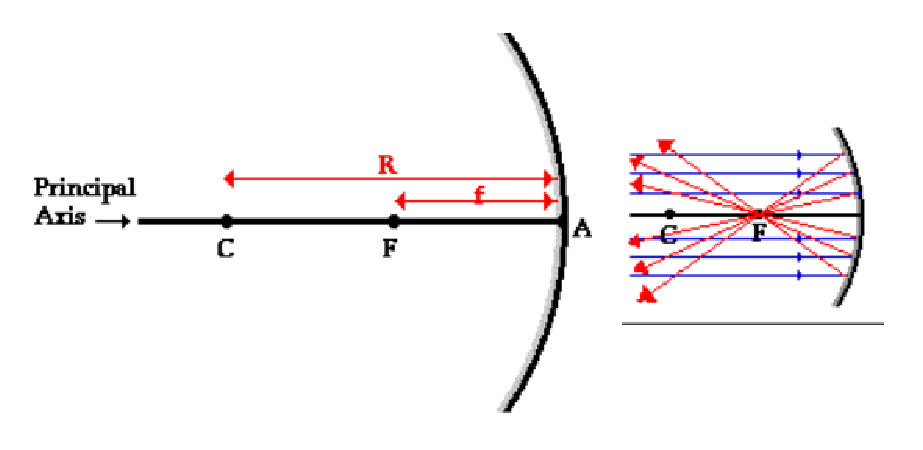
\includegraphics[height=4cm,
    angle=0]{./images/light_curvature.eps}}    
\caption{Curvature mirror}
\label{fig:light_curvature}
\end{figure}

The lens is an object that allows the light to go through, and it can bench the
light. Depending on the material of the lens, the {\bf Diopter value} tell how
much the lense can bend the light, i.e. refractive power.
\begin{verbatim}
Diopter = 1 meter / (Focal length)
\end{verbatim}
Ideally, the lense can
bend the light coming from infinity, i.e. the Diopter value is zero. 
A diopter value is widely used than {\bf focal length}, as it can be added when
putting multiple relatively thin lense together, the overal refractive power is
the sum of that of all lenses. A human with good eyes generally has total
Diopter value from 58 to 59. So
\begin{verbatim}
Focal length = 1 meter / 58 = 17.24 mm
Focal length = 1 meter / 59 = 16.9 mm
\end{verbatim}
The cornea accounts for about 2/3 of this refractive power, and the crystalline
lense in conjunction with the aqueous contributes the remaining third. 

% The diopter value is from -14 to 14 for human eye. For young, it's from 15-20
% diopter; and 10 at ages of 25, and around 1 at 50 or over.





\section{Human eye vs. Camera}

\begin{figure}[hbt]
  \centerline{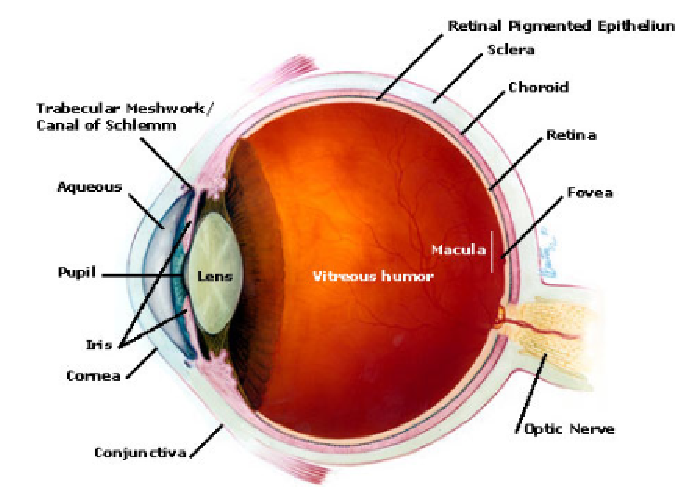
\includegraphics[height=6cm,
    angle=0]{./images/eye1.eps}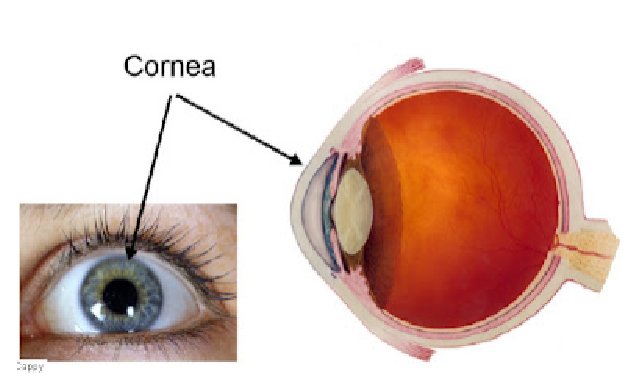
\includegraphics[height=4cm,
    angle=0]{./images/human_eye.eps}}    
\caption{Eye}
\label{fig:eye}
\end{figure}

The human eye is composed of 3 layers, Fig.\ref{fig:eye}:
\begin{enumerate}
  \item outermost layer: sclera (the white tough wall of the eye) and cornea
  (in the front)
  \item middle layer: choroid (containing vascular tissue lining between retina
  and sclera), ciliary body, and iris
  \item innermost layer: retina
\end{enumerate}


A {\bf cornea} is a transparent structure, covering the very front of human eye
that help to focus incoming light. The shape of a cornea is best represented as
an ellipse. It functions as the extended lens being used in DSLR camera. So, a
human eye can be considered as a typical camera with a cornea. In high-end
camera, a wider lense can be used to collect more lights coming from wider view.

Then comes an {\bf iris} which is not spherical shape, but a fused two-piece
unit and it is used to take widely diverging rays of light from many directions
(as wide as 120-200$^\circ$ angle of view) and bend it to the {\bf pupil} which
is at the center of a ring-shaped membrane called pupil. The pupil is an
adjustable circular opening (hole). {\it The iris is like the aperture of a
camera}.
It adjusts to control how much light entering the eye so that the eye can work
well with a wide range of light brightness.

In the camera, when you press slightly and hold the button on the camera, a hole
opens up and allow your camera sensor to catch a glimpse of the scence. The size
of that hole is defined via the concept {\bf aperture}, measured in `f-stops' or
f/(number), e.g. f/2.8, f/5.6, f/22 \ldots Moving from one f-stops double or
half the size of the hole. Besize the size of the hole, there is another term to
reflect the opening time of the hole called {\bf shutter speed} (to be discussed
later). A larger aperture gives a lot of light get through, and correspond to a
smaller f-stop number. In human, f-stop can vary from f/8.3 (very bright light),
to f/2.1 (in the dark).

The {\bf retina} contains photoreceptor nerve cells that can sense light of
different wavelength. When the light strike these nerve cells, the cells transmit the
proper signals to the brain where an image is perceived. The retina has 2 types
of photoreceptors: cones and rods. Cones is responsible for colour vision, but
much less sensitive to low light than the rods ({\bf photopic vision}). The 10\%
of the retina, i.e.
the macula, is responsible for your sharp vision
\footnote{\url{http://www.pasadenaeye.com/faq/faq15/faq15_text.html}},
Fig.\ref{fig:eye}.

{\it The retina is like the ISO number of the camera}. To quantity how sensitive
to the light of a digital sensor, we use the term {\bf ISO number} (film
speed)\footnote{\url{http://digital-photography-school.com/iso-settings}}. It's
measured in number like 100, 200, 400, 800,\ldots. The higher the ISO, the more
sensitive to light, but at a cost of a larger amount of digital noise. In order
to capture image with low light, we need camera that supports high ISO. At
normal light, ISO = 100 is good. In bright light condition,
the range of wave length is wide, so a small change in wavelength (i.e. noise)
is not affecting much to the image. In dim light condition, the range of wave
length is short, so a small change in wavelength is amplified. So, when this
change is caused by the noise, it affects the resulting image.


\begin{framed}

\textcolor{red}{Higher ISO is used to take picture in low light condition or
capturing moving objects}. With higher ISO, as the time exposing to the image is
short, it can be vulnerable to noise, and to avoid bluring, you use (1) tripod,
(2) higher shutter speed and/or smaller apertures.

For a picture that is take good at ISO 100, if you use ISO 400, you only need
1/4 of the light to get the same quality picture. So, use higher ISO when the
light is low \footnote{\url{http://www.pixiq.com/article/eyes-vs-cameras}}. We
also tend to use higher ISO when an object is moving, as higher ISO has higher
shutter speed. In fact, a camera can stay open for as long as we need to, i.e.
use very low ISO.

Scenarios to use high ISO: indoor sport events, concerts, birthday parties, art
galleries\ldots
\end{framed}

When you enter a dark room, the pupil expand (larger hole or smaller f-stop
number) to receive more lights. For the eye, if you stay long enough in the dark
room (about 30mins), there are chemical adaptations making the rods become more
sensitive to dim light, at about 10,000th of the level needed for the cones to
work. However, we don't have good colour vision in the dard. The human eye can
distinguish about 10 million colors. 

\begin{framed}
In photography, the three important things is ISO, shutter speed and aperture.
They are collectively called {\bf the exposure
triangle}\footnote{\url{http://digital-photography-school.com/learning-exposure-in-digital-photography}}.
\begin{enumerate}
  \item ISO : measure digital camera sensor's sensitivity to light (the lower
  ISO, the less sensitive to light and thus the finer the grain).
  \item Aperture : the size of the opening in the lens when a picture is taken
  \item Shutter speed: the amount of time (in sec) that the shutter is open.
  Typically, it's represented in the form 1/n, e.g. 1/60th or faster is
  typically used in most cases. Anything slower, i.e. 1/60th or smaller
  denominator, we need to use a tripod. 
  
  The typical settings are 1/500, 1/250, 1/125, 1/60, 1/30, 1/15, 1/8th.   
\end{enumerate}
A change in one element will affect the others. Another quantity is {\bf focal
length} 
\end{framed}

{\bf Shutter speed} is the amount of time (in second) that the shutter is open.
In most cases, the shutter speed of 1/60th of a second or faster is used. 
If you use a slower shutter speed, to avoid image blurring, then you need to
have a tripod or some type of image stabilization (new cameras have this feature built-in). What
is the role of {\bf shutter speed}? Imagine that you capture a moving object, if
you open your eyes long enough, you'll have the feeling of that object is
moving. If you open and shut your eye instantly, you can capture one instant of
that object and thus avoid the blurring effect. The same thing, you need to
capture fast enough to get a good picture of a moving object.
So, we need high shutter speed when capturing moving objects or using small.

Another quantity is called {\bf numerical aperture} (NA) that tell the range of
angles over which the system can accept light
(Sect.\ref{sec:numerical_aperture}).
NA is not typically used in photography, but the f-number (written as f/\# or N).
\begin{verbatim}
f-number = f / (diameter of entrance pupil)
\end{verbatim}
with $f$ is the focal length, Fig.\ref{fig:NA_f-number}. If you want to create
the motion effect, set a low shutter speed.  

% Another factor affects image
% blurring is {\bf focal length} (to be discussed later).

\begin{figure}[hbt]
  \centerline{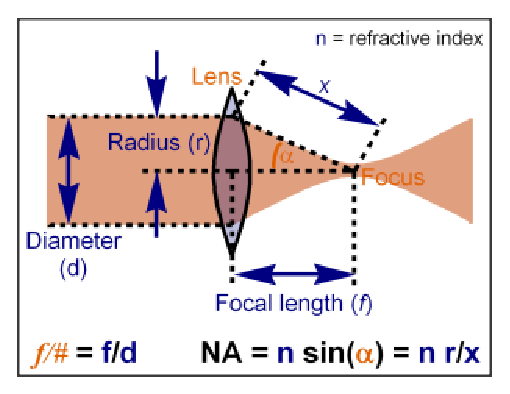
\includegraphics[height=6cm,
    angle=0]{./images/NA_f-number.eps}}    
\caption{ Calculate NA and f-number}
\label{fig:NA_f-number}
\end{figure}

\begin{framed}
Even though the eye is very sensitive (the rods can respond to a single photon),
to avoid 'visual' noise, in order a signal to trigger a brain conscious
response, at least 5-9 photons need to arrive within less than 100ms
\footnote{\url{http://math.ucr.edu/home/baez/physics/Quantum/see_a_photon.html}}
({\bf scotopic vision}).
\end{framed}

When you capture a scence, you can also define how large of the area will be
in-focus, the other parts will be fuzzy. This is reflected via the concept of
{\bf depth of field} (DOF). A small (or shallow) DOF means only a part is in
focus. Aperture has a big impact on DOF, i.e. large aperture (i.e. small
f-stop number or small hole) give small DOF and vice versa. 

{\bf Field of view} (FOV) tells you how wide of the area that an eye can
perceive from a single point. The farther that point, the wider the view; and
also the less detailed that you can perceive, Fig.\ref{fig:FOV}. A numerical
value to represent FOV can be angular A (in degrees) or linear L (ratio of
lengths).

\begin{figure}[hbt]
  \centerline{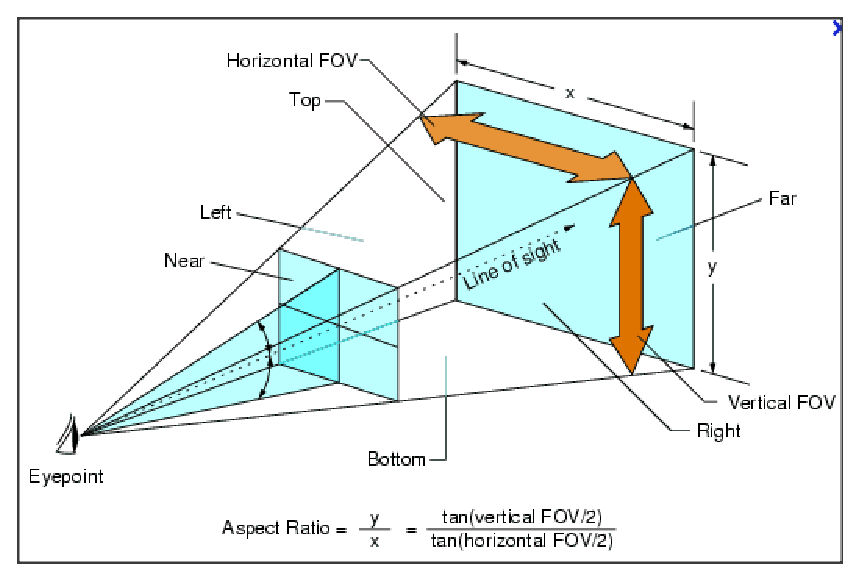
\includegraphics[height=6cm,
    angle=0]{./images/field_of_view.eps}}    
\caption{FOV}
\label{fig:FOV}
\end{figure}

Human eye is of length 24.5 mm from the front to back. So, all the lights
entering the eye has less than 24.5 mm to converge the focus. It means that the
focal length should be less than that. As pointed above, the focal length of a
normal human eye is from 16.9 mm to 17.24 mm. 

To help capture the image as sharp as possible, we need to use a proper lense. A
lense that help directing the focusing the light to produce an image is called
{\bf objective lense}. A camera (objective) lense help direct the light rays as
accurately as possible on the digital sensor
to
minimize
aberrations\footnote{\url{http://www.cambridgeincolour.com/tutorials/camera-lenses.htm}}.
A lense can be of different shapes, Fig.\ref{fig:lense_shape}. A camera lense
can be an assemble of multiple lenses. 

\begin{figure}[hbt]
  \centerline{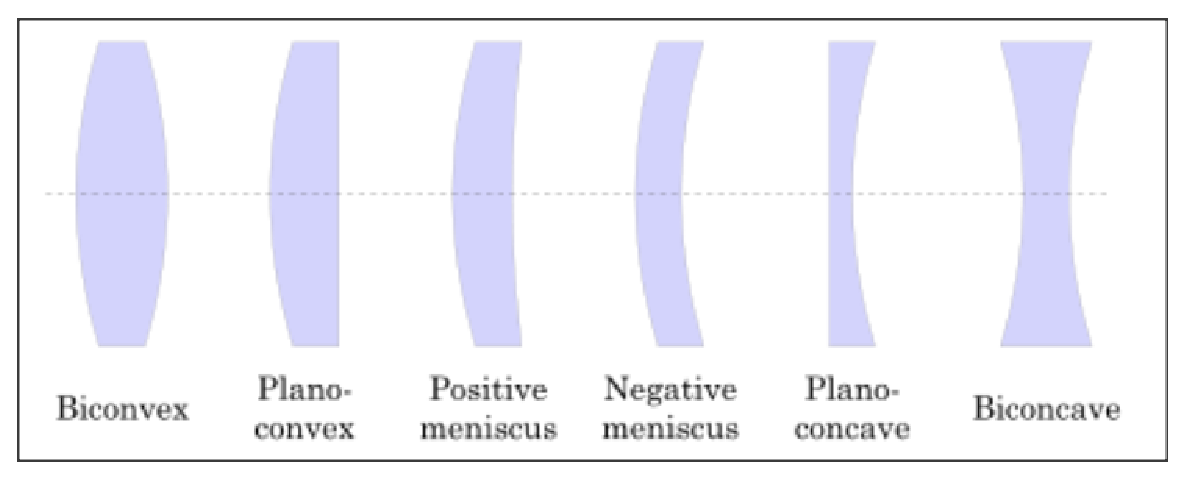
\includegraphics[height=4cm,
    angle=0]{./images/lense_shapes.eps}}    
\caption{Lenses}
\label{fig:lense_shape}
\end{figure}

\section{Focal length $f$}

A focal length $f$ of a lense is calculated based on (NOTE: we don't use $f$,
but $1/f$ as we can easily sum the Diopter value when we combine multiple lense
to increase the power)
\begin{equation}
1/f = (n-1)\left[ \frac{1}{R_1} - \frac{1}{R_2} +
\frac{(n-1)d}{nR_1R_2} \right] 
\end{equation}
with $n$ is refractive index of the lens material; $d$ is the thickness of the
lense, $R_1$ is the radius of the curvature of the lense at the side closest to
the light source. NOTE: $R_1$ is positive if the corresponding surface is convex
and vice versa; $R_2$ is positive if the corresponding surface is concave and
vice versa. 

The approximation (when $d \ll R_1, R_2$)
\begin{equation}
1/f \approx (n-1)\left[ \frac{1}{R_1} - \frac{1}{R_2} \right]
\end{equation}


Optical aberrations occur when a point on the object is not translated to a
single point on the picture, causing image blurring, reduced contrast or
misaligned of colors (aka chromatic aberrations). Other problems include
unintended darkening of the image toward the corners (aka vignetting) or
distortion. To resolve this, a camera lens is composed of multiple thin lenses,
Fig.\ref{fig:camera_lens}.

\begin{figure}[hbt]
  \centerline{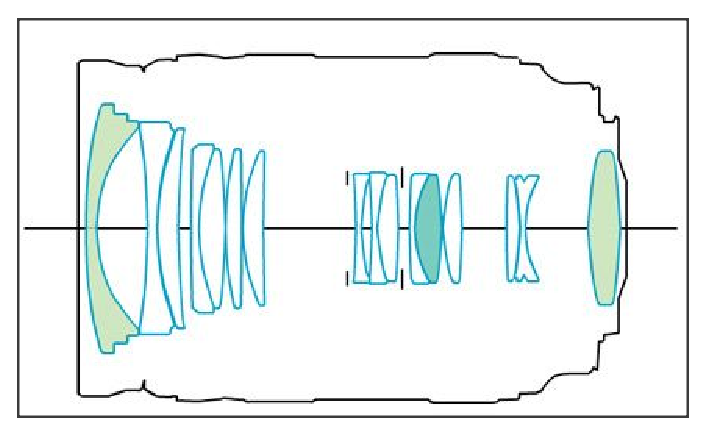
\includegraphics[height=4cm,
    angle=0]{./images/camera_lens.eps}}    
\caption{Camera lenses}
\label{fig:camera_lens}
\end{figure}


\begin{framed}
  The focal length of the lens is $F$, and the magnification of the
  objective $M$ gives the {\bf focal length of the objective}
  $f=F/M$. 

  For aberration-free lens, the ray leaving the focus at an angle
  $\alpha$ to the optical axis is intercepted by this surface at the
  height $d=f\sin\alpha$. For immersion lens, this has to be
  multiplied by a refractive index of the immersion fluid $n$. 

  NOTE: $n\sin\alpha$ is known as numerical aperture (NA). The
  objective lens $D$ is
  \begin{equation}
    \label{eq:1112}
    D = \frac{2Fn\sin\alpha}{M}
  \end{equation}

\end{framed}



% Human eye has a spherical shape to focus incoming light.

% 
% Remember that light is has dual wave-particle properties. What if the light
% approach the edge of the surface (or small obstacle)? Answer: the light bending
% around small obstacles. What if the light go through small holes, i.e. the width
% is about the wavelength? Answer: the light is spreading. So, by studying the
% diffracted light, we can learn something about the geometry of small objects.
% One of the first successful application was to study DNA double-helix structure
% using X-ray diffraction.
% 
% 	
\section{Numerical Aperture (NA)}
\label{sec:numerical_aperture}

Typically, a fiber cable is composed of a fiber optics with refractive index
$\eta_1$, surrounded by one or more layers of lower refractive index,
Fig.\ref{fig:numerical_aperture}.
These layers are called {\bf cladding} and is in intimate contact with the core.
Suppose there is a single cladding with refractive index $\eta_2$. This
numerical aperture (NA) is defined as
\begin{equation}
\text{NA} = \sqrt{\eta_1^2 - \eta_2^2}
\end{equation}
This dimensionless number can tells the range of angles the system can
receive/emit lights. In microscopy, NA is defined differently
\begin{equation}
\text{NA} = \eta \sin(\theta)
\end{equation}
with $\eta$ is the refractive index of the medium in which the lens is working
on (1.0 for air, 1.33 for pure water, 1.47 for glycerin, and 1.51 for immersion
oils), and $\theta$ is the maximum angle from the center of the cone axis. 

\begin{figure}[hbt]
  \centerline{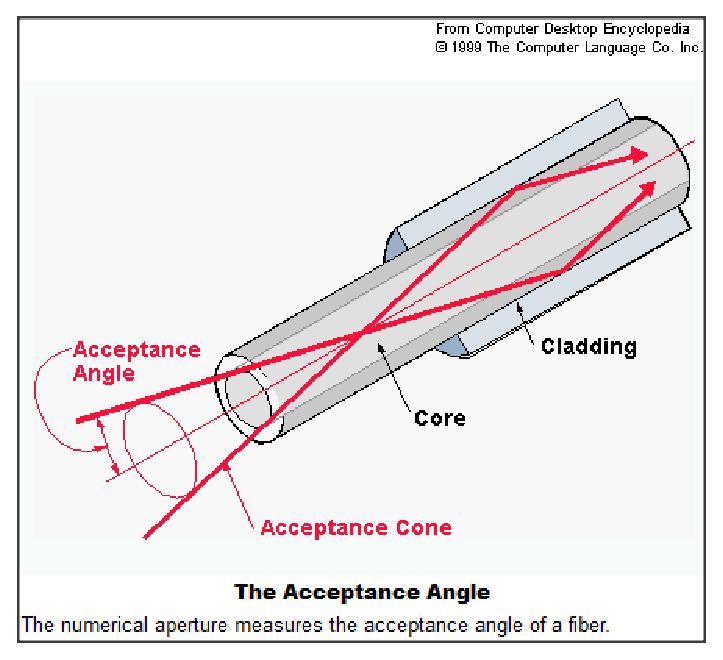
\includegraphics[height=4cm,
    angle=0]{./images/numerical_aperture.eps}}    
\caption{Numerical Aperture (N/A)}
\label{fig:numerical_aperture}
\end{figure}

Similar to optical fiber, in a microscope, it can only receive the ligth from a
particular angle from the core axis, Fig.\ref{fig:NA}. If the medium is air
(i.e. dry objectives with $n=1$), then the maximum value for NA is 1.0. In
practice, it's difficult to achive NA $>$ 0.95 with dry objectives. Also, the
angle is smaller than 90$^\circ$. The practical upper limit is about 72$^\circ$
(with a sine value 0.95).


\begin{figure}[hbt]
  \centerline{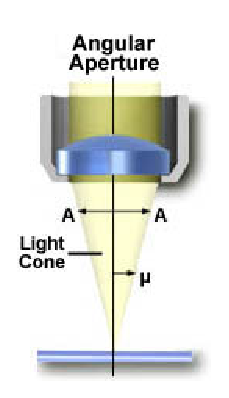
\includegraphics[height=5cm,
    angle=0]{./images/NA.eps}}
  \caption{numerical aperture
  (NA)\footnote{\url{http://micro.magnet.fsu.edu/primer/anatomy/numaperture.html}}}
  \label{fig:NA}
\end{figure}

For alternate medium like immersion oil, the
most common NA is from 1.0 to 1.35 (though maximum NA is 1.4). The higher the
NA, the greater light gathering capability which make the resolution higher. 

There are two things that determine the quality of a microscope to resolve small
specimens are:
\begin{enumerate}
  \item NA 
  \item wavelength: it can resolve any speciment smaller than half of the
  wavelength being used.
\end{enumerate}



\section{Single-molecule imaging}

\subsection{Scientific goal}

Single-molecule spectroscopy (SMS) and imaging experiments measure signals from
each individual fluorescent label in living cells. We can measure the full
distribution of experimental parameter instead of from a single population
average, which allows us to expose normally hidden heterogeneities in complex
systems \citep{lord2010}. Stuyding living cells can be significantly more
difficult than {\it in vitro} or fixed cells, as the environment exhibit
continually changing states.

Green fluorescent protein (GFP) derived from jellyfish {\it Aequorea victoria}
and its mutants are widely used biological labels as the fluorephore can be
formed {\it in vivo} \citep{dickson1997}. Wild-type (WT) GFP has 2 absorption
maxima: strong peak at 396nm and a weak peak at 476nm; and only one emission
maxima: 508nm. The two popular yellow-fluorescent GFP mutants are:
S65G/S72A/T203F (denoted T203F) and S65G/S72A/T203Y (denoted T203Y).


\subsection{Cell preparations}

We need a transparent, nonfluorescent host matrix. A molecule that can be
separated should be larger than the diffraction limit of $\sim 200$nm. To avoid
autofluorescent (from endogenous cellular fluorophores like flavins, NADH,
tryptophan), an imaging wavelength should be longer than about 500nm, and/or
using cell growth media and imaging buffers with free of fluorophores.

To introduce the probe into the cell across the membrane, we should use a
genetically expressed or membrane-permeable probe; or we have to use
microinjection or electroporation. 

For targetting the organic fluorophores to biomolecules of interest in the cell,
bio-orthogonal labelling reactions are necessary. Then, another challenge is
washing out unbound copies of probes introduced into the cell. Lastly, but not
less importantly, the experiment should not significantly interfere with the
relevant biology of the cell.

Example: \citep{cui2007} used single QD to label nerve growth factor (NGF) and
track their transport in the axon of a living neuron, i.e. quantum dot-labeled
NGF (QD-NGF). Previously, the mechanism of how NGF signal is propagated from the
axon terminal to the cell body is poorly understood. This lead to the
understanding that a single NGF dimer is sufficient to initiate signaling. 

Example: To study membrane constituents and organizations, they probed tiny
regions on the membrane to search for heterogeneous dynamics by tracking single
proteins's diffusion \citep{kusumi2005}. The frame rate can be as high as 40
kHz, and it showed hop diffusion between submicrometer regions, suggesting a
heterogeneous structure known as {\bf lipid rafts} in the membrane, or {\bf
picket fence} model of membrane rafts \citep{kusumi1996}.

Fast motion protein can become blurring into the background at even the fastest
readout speed of CCD cameras.  To track fast protein motion


\subsection{Techniques}

\citep{hirschfeld1976} presented the first single-molecule fluorescence imaging
at room temperature. The method reduced the detection volume to enhance
signal-to-background noise ratio. An example if an (immobilized) protein
(cholesterol oxidase molecule E) which has a flavin moiety that is naturally
fluorescent in oxidized form (FAD), but not in reduced form (\ce{FADH2}),
Fig.\ref{fig:hirschfeld1976}. So, whenever the protein is oxidized, it can be
detected. The image shown that this is a stochastic process. Even the binding
occurs very fast (less than 1ps), the waiting time is much longer and is
probabilistic and thus can be detected. The ability to control fluorescent
proteins (FP) photoswitching was demonstrated in \citep{dickson1997}. 

\begin{figure}[hbt]
  \centerline{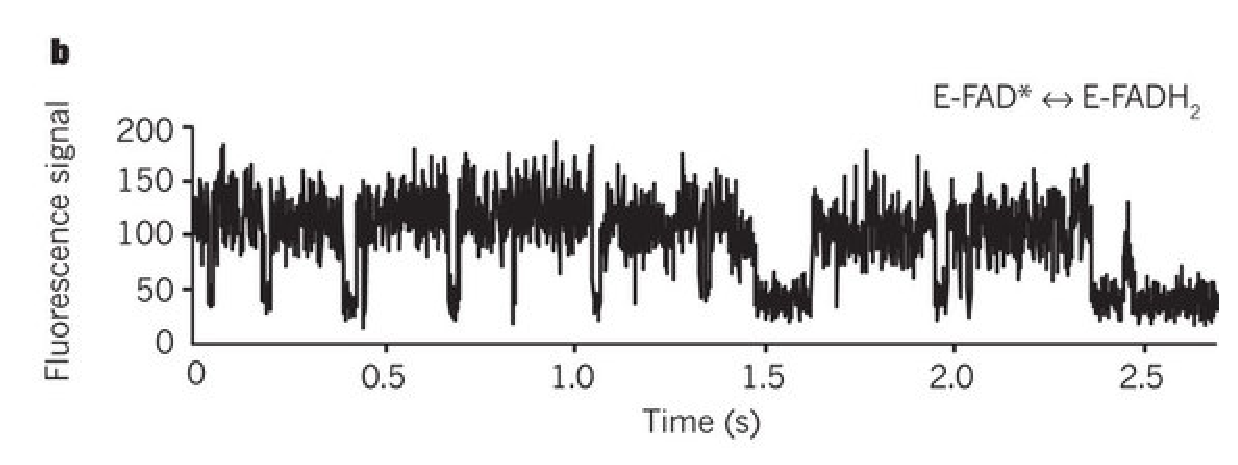
\includegraphics[height=4cm,
    angle=0]{./images/protein_fluoscent_hirschfeld1976.eps}}
\caption{}
\label{fig:hirschfeld1976}
\end{figure}


In a reaction with rate-limiting step, the distribution of
waiting-time follows a single exponential distribution, and the number of events
in a fixed time interval follows a Poisson distribution.
Otherwise, i.e. it consists of identical sequential steps, the total waiting
time is less stochastic \citep{li2012}. Transcription-factor binding
to/unbinding from DNA is a rate-limiting event. 

Stochastic binding/unbinding of transcription factors to a particular gene, when
rate limiting, must result in stochastic mRNA production. Then, stochastic
degradation of individual mRNA molecules further contributes to fluctuations in
protein production. This results into cell-to-cell variation in the number of
proteins in each cell (copy numbers), or gene expression 'noise'. 

In a cell, the copy number of a particular protein range from zero to 10,000.
Many important proteins, like transcription factors (that regulate gene
expressions), have small copy numbers. Also, the short lifetime of intracellular
mRNA amplifies the importance of single-molecule tracking technique at real-time
observation. 

To record a single protein, specific labelling is required. Nowadays, we can
have genetically encodable fluorescent proteins (FP) \citep{giepmans2006}.
Popular organic fluorophores:
Cy3, carbocyanine dyes, rhodamines, fluoresceins, DCDHF
(dicyanomethylenedihydrofurans), teryline and rylenes. Other choices are
photo-switchable or phoactivatable probes: Cy3-Cy5 pairs, DCDHFs, rhodamines,
merocyanines.  The technique: strong but noncovalent binding to short peptide
motif using FlAsH-type fluorophores can be used {\it in vitro}, but has some
problems of off-target labelling and low photostability {\it in vivo}.

The weak signal of a single fluorescent-protein can be detectable
using modern charge-coupled device (CCD) detectors to amplify the signal and
reduce the probe volume. To avoid strong cellular autofluorescence, the
fluorescent proteins need to have a separate spectral from autofluorescence
\citep{andersson1998}.  Autofluorescence is generally blue-green; so yellow or
red-emitting fluorescent proteins are favourable for live-cell single-molecule
imaging.


\begin{figure}[hbt]
  \centerline{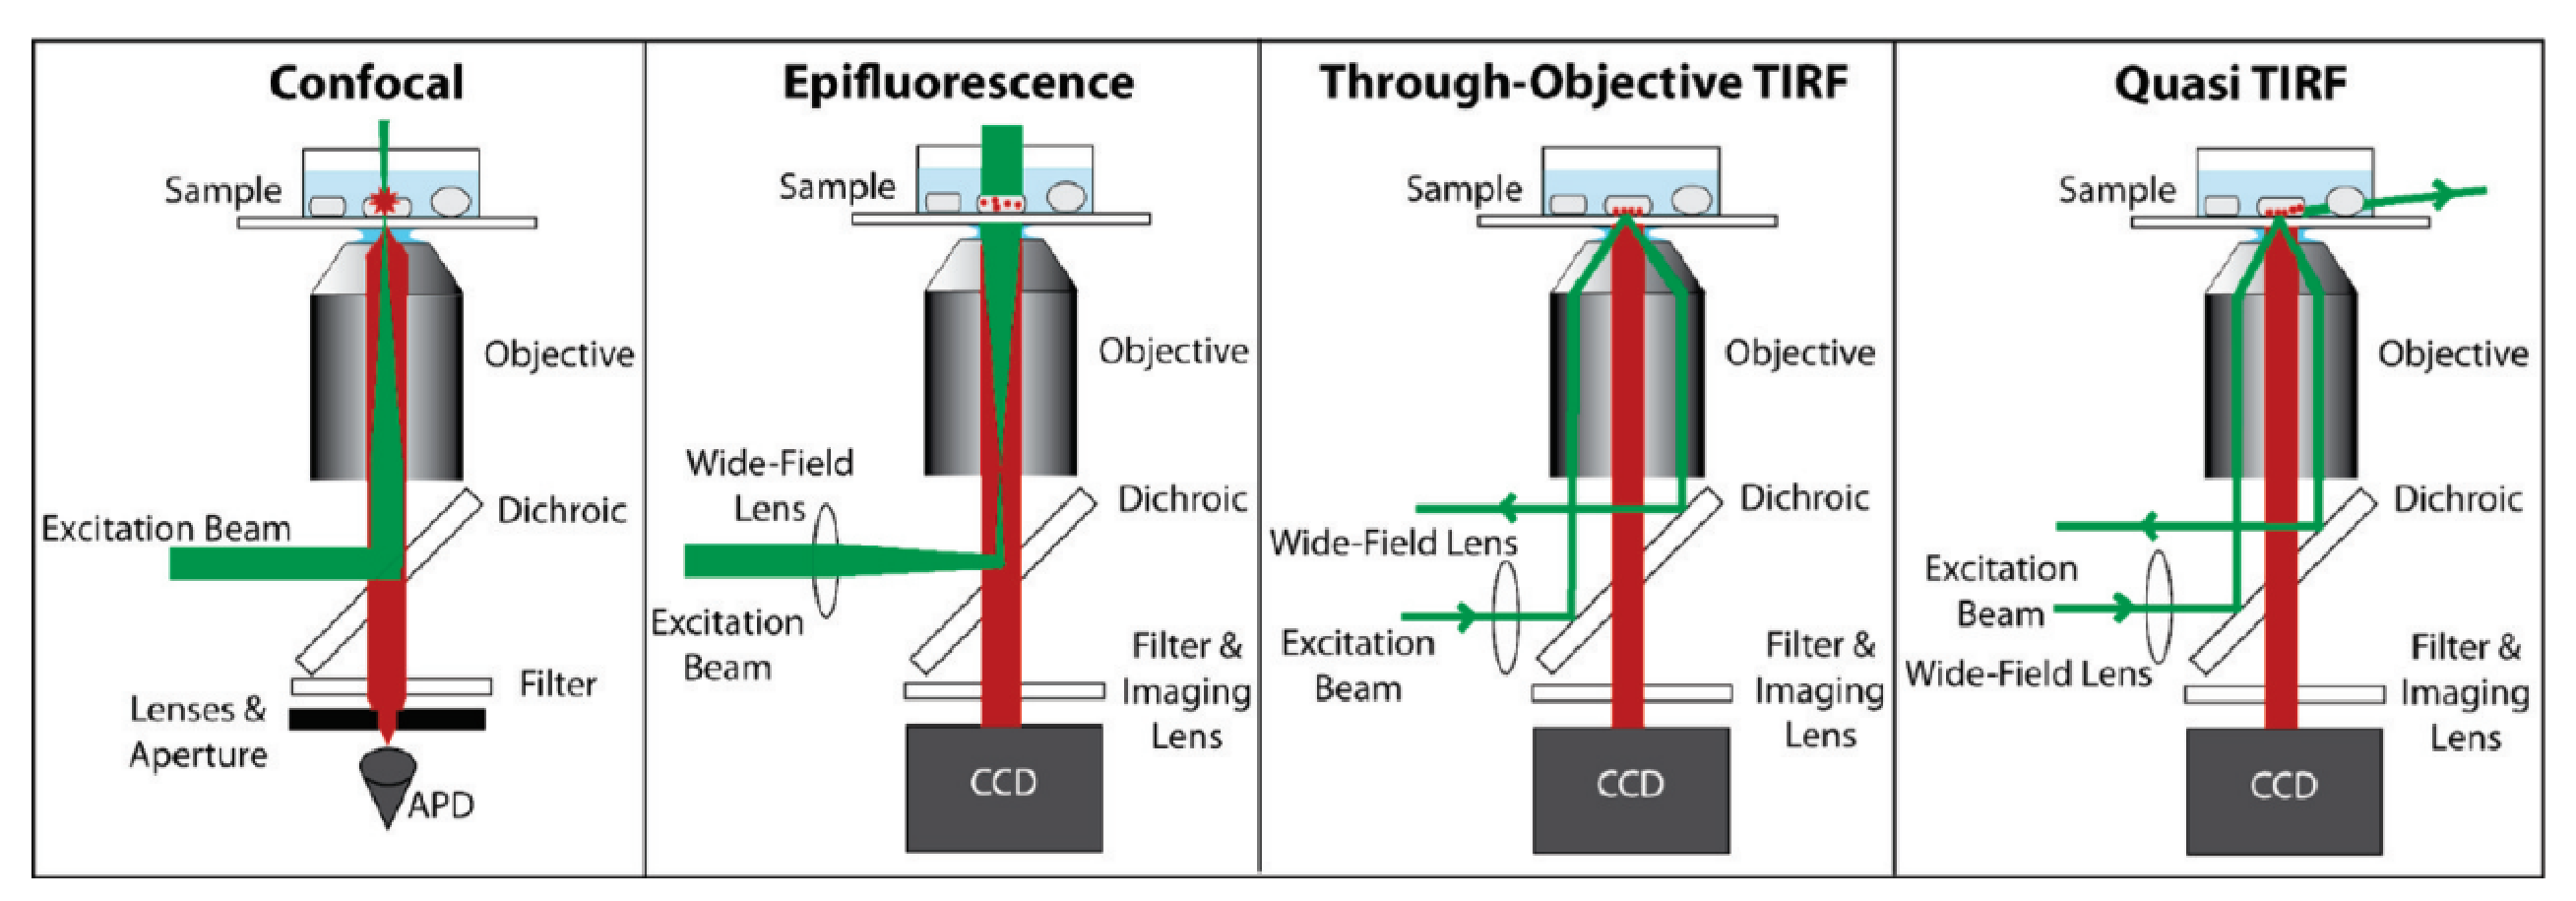
\includegraphics[height=4cm,
    angle=0]{./images/imaging_techniques.eps}}
\caption{}
\label{fig:imaging_techniques}
\end{figure}

Inverted optical fluorescence microscopes (configured in either wide-field
illumination or confocal imaging) can be used to record single-molecule imaging,
Fig.\ref{fig:imaging_techniques}. Epifluorescence is the simplest wide-field
method, i.e. an excitation beam (in green) is focused o nthe back focal plane of
the objective, producing a collimated illumination beam (in red) which is then
filtered from out-of-focus signal using a dichoric mirror and long-pass or
bandpass filter, before imaged onto the camera. The drawback is a large volume
of sample is excited. To overcome, TIRF is a method of choice, or a variant
called quasi-TIRF (pseudo-TIRF or leaky-TIRF). Another method to overcome
out-of-focus signal is confocal imaging (i.e. point-detection or scanning
technique). Confocal imaging can be used to image deep into the sample or for 3D
imaging. 

Point detector for confocal imaging can be: PMT (photomultiplier tubes with
large detection area $\sim 1$cm$^2$ and picosecond to nanosecond in time
resolution), APD or SPAD (avalanche photodiodes with small detection area and
very low dark counts (better detect single photons), faster time resoltuion), or
hybrids thereof. Due to small detection area of APD, it makes aligning onto the
sensor more difficult. Wide-field can use multi-detector arrays or cameras like
CCD (charge-coupled devices). Modern Si CCD often include on-chip electron
multiplication to increase sensitivity and reduce noise. Faster imaging rates
(10-100ms) can be achieved using frame-transfer technology by performing the
slow readout step on a separate dark section of the chip. 

 \begin{figure}[hbt]
  \centerline{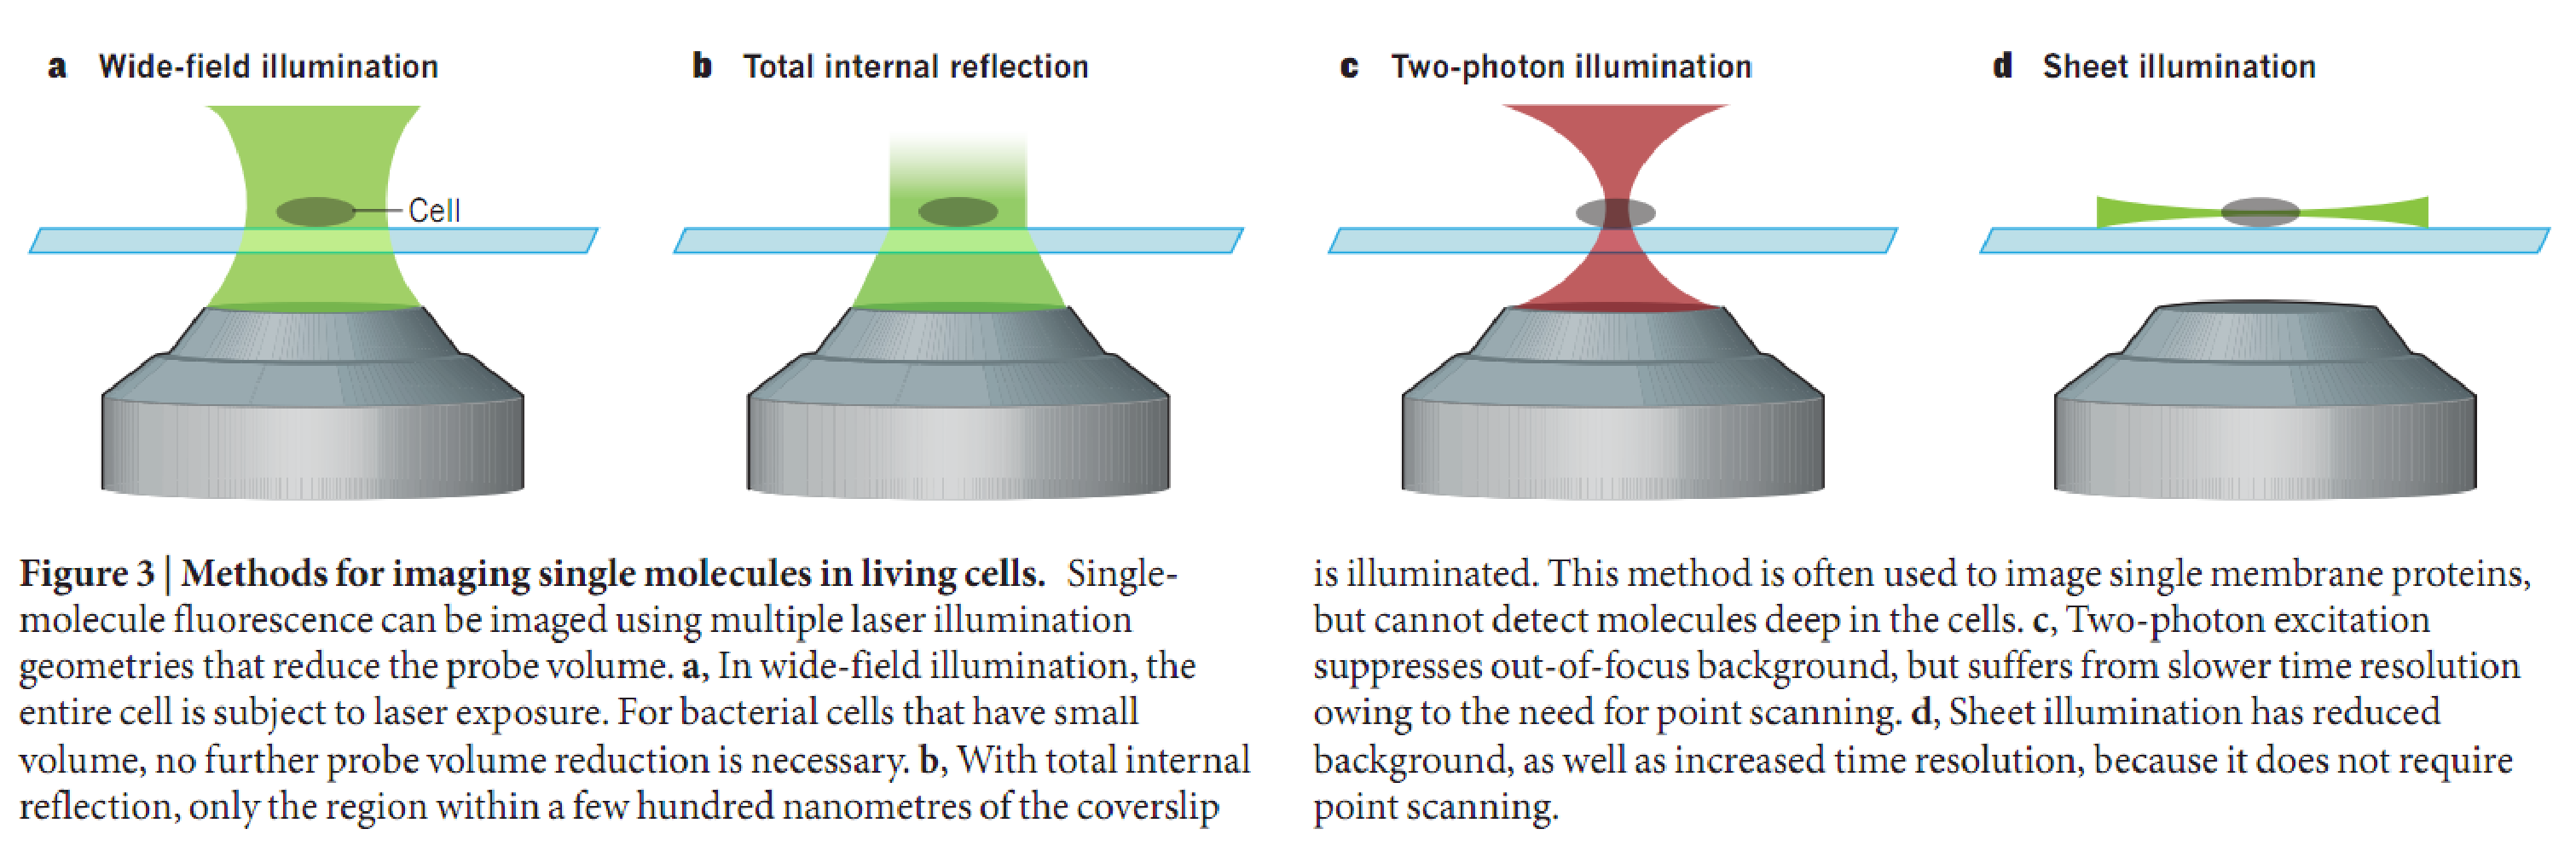
\includegraphics[height=4cm,
    angle=0]{./images/single_molecule_imaging.eps}}
\caption{Methods for imaging single molecules in living cells}
\label{fig:single_molecule_imaging}
\end{figure}

Immersion objectives with high numerical aperture (N.A. $\sim 1.4$) are used to
collect as much of the emission as possible but can complicate polarization. 

\begin{enumerate}
  \item TIRFM (total internal reflection fluorescence microscopy): the technique
  to limit the axial depth (i.e. reduce the detection volume to minimize
  autofluorescence background) by illuminating with an evanescent wave that
  penetrates only a few hundred nanometres into a sample. CONS: it works well
  only at the surface (membrane proteins), but not allow imaging the whole cell
  body. For bacteria with compact sizes (with nucleus $1\mum$), the technique
  can also be used.
  \item Two-photon microscopy: work for typical mammalian nucleuus 5-10$\mum$ in
  diameter. The technique allows localized excitation only at the laser focus,
  i.e. reducing out-of-focus photobleaching while providing 3D sectioning in
  living eukaryotic cells. CONS: it requires point scanning, thus limiting its
  time resolution.
  \item Sheet illumination (use a thin light sheet to illuminates an image
  plane): to records a whole area, i.e. no need for point scanning. 
\end{enumerate}




\section{Point-Spread Function}
\label{sec:PSF}

% Ideally, a photon counts detected from a focal point (ie. bead) is mapped into
% the intensitity of a single pixel in the digital image. However, the image of a
% point source along the axial plane, without a hole, is not a point, but has an
% hourglass shape with the smallest point being at the focal point of the lens,
% Fig.\ref{fig:PSF_axial}. Without a pinhole, the noise of photons from
% neighboring area occur. This means that the PSF is not a sphere as the axial
% dimension is larger than the lateral dimension.
% So, the axial (Z) direction is not as good as that in the lateral (X-Y) plane.

The microcope captures a small object and produce a magnified picture of it.
Ideally, one point on the object is mapped to a sharp pixel in the image.
However, due to diffraction of light, the image is always blur. The image of a
focal point (i.e. a bead) is mapped to an image whose intensities of the pixels
resemble the 3D intensity distribution. The size of the PSF determines the
resolution of the microscope. 

The property of the intensity point spread function (PSF) in the image plane
(lateral direction) and axial direction are major factors determining the
resolution of the microscope. Although PSF extends in 3D, we can consider only
the lateral component, with reference to the familiar {\bf Airy disk}. The two
lateral components (x and y) of the Airy pattern are equivalent, due to the
cylindrical symmetry of the microscope lenses. \textcolor{red}{Airy disk is the
2D paraxial WFFM PSF} (Sect.\ref{sec:PSF_WFFM}).

\begin{figure}[hbt]
  \centerline{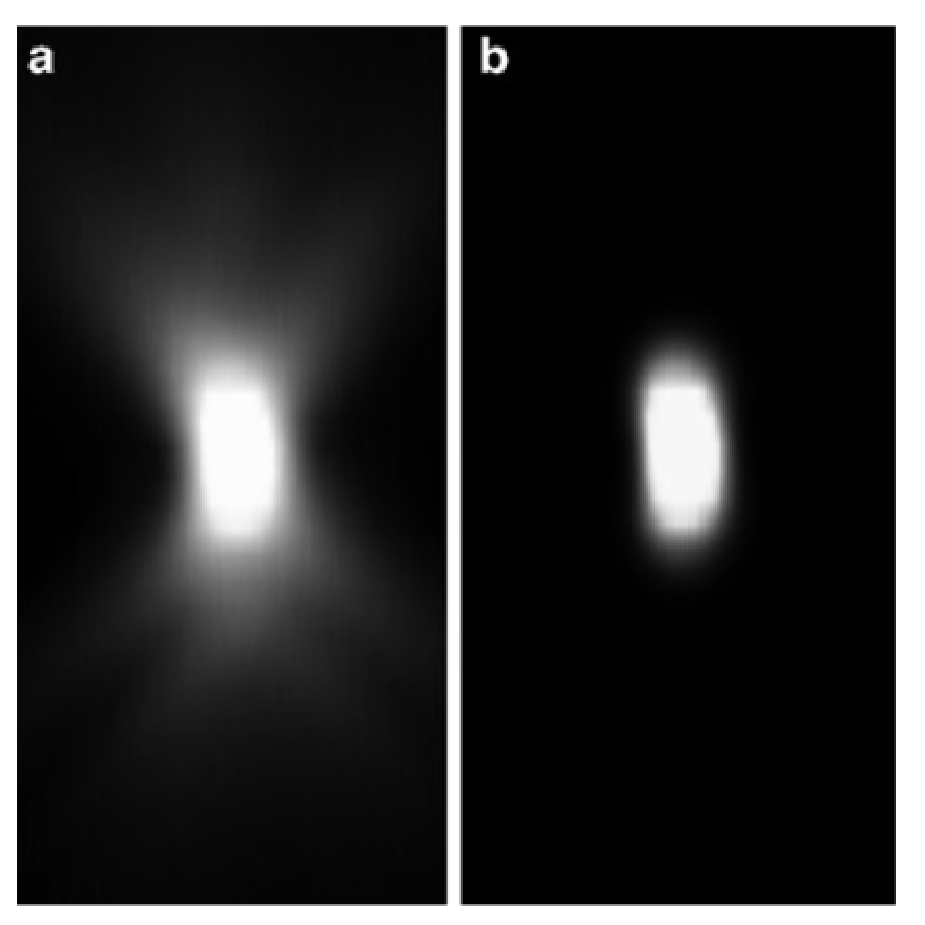
\includegraphics[height=6cm,
    angle=0]{./images/PSF_axial.eps}}
  \caption{PSF of a 0.15-$\mum$ bead which is imaged in X-Z (axial) plane. (A)
  without a pinhole, and (B) with a pinhole set to 1 [Airy unit]}
\label{fig:PSF_axial}
\end{figure}

PSF is the response of the optical system to a point in the objective plane. To
approximate PSF, a tiny small object is used as an ideal point, and the system
record the signal from the small object, which can be colour bead or the like.

\subsection{FWHMs of PSF}

As mentioned in Sect.\ref{sec:resolution_limit}, the FWHM of the PSF in the
lateral direction can be approximated by
\begin{equation}
FWHM \approx \frac{0.61\lambda}{\text{N.A.}}
\end{equation}
The axial width of FWHM is about 2-3x. When imaging with visible light
($\lambda=550$nm), and oil-immersion objective lens N.A.=1.40, it gives a PSF
with lateral size 200nm and axial size 500nm

The PSF also change at different wavelengths, e.g. N.A.=1.4 lens
in a system using immersion oil with $\eta=1.515$, the lateral and axial PSF is
\begin{enumerate}
  \item blue (442nm): 0.129$\mum$ (X-Y), 0.478$\mum$(Z)
  \item green (541nm): 0.158$\mum$ (X-Y), 0.585$\mum$(Z)
  \item red (690nm): 0.202$\mum$ (X-Y), 0.747$\mum$ (Z)
\end{enumerate}
NOTE: Reducing the pinhole below 1 [Airy unit] produces little gain in the axial
resolution, but does significantly decerase the number of photons passing
through the aperture. On the other hands, increasing the pinhole, allows more
photons passing, including those from out-of-focus regions, which blur the edges
of objects which degrades both the lateral and axial resolution.


\begin{framed}
Confocal microscope has FWHM reduced by about 30\% compared to that of wide-field
microscope. So, the value is 
\begin{equation}
r_\text{lateral} = 0.4\lambda/\NA
\end{equation}
This is for lateral resolution. How about axial extend? A: it's similarly
reduced in the confocal arrangement compared to the wide-field fluorescence
configuration, Fig.\ref{fig:axial_PSF}. For the axial, the formula is different
\begin{equation}
r_\text{axial} = 1.4\lambda\eta/(\NA^2)
\end{equation}
which is a function of wavelength, refractive index of the specimen medium
$\eta$, and inversely proportional to the square of the NA. So, the NA has a
much greater effect on axial resolution compared to wavelength. 

\end{framed}

\begin{figure}[hbt]
  \centerline{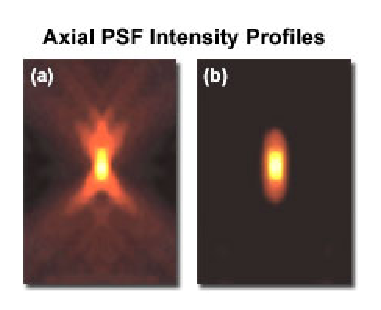
\includegraphics[height=5cm,
    angle=0]{./images/microscope_axial_extent.eps}}
  \caption{The PSF in axial extent in (A) wide-field microscope; (B) confocal
  microscope. NOTE the reduce in intensity of the ``wings" as a function of
  distance from the center maximum in confocal
  microscope\footnote{\url{http://www.olympusconfocal.com/theory/resolutionintro.html}}}
  \label{fig:axial_PSF}
\end{figure}



\subsection{Mathematical Formula: PSF}

By definition, PSF is the product of the excitation intensity distribution
(characterized by the emitted light), and [ the emission intensity
distribution (generated by the fluorescence) convolved with the area of
the detector ]
\begin{equation}
\PSF (x,y,z) = |h_{ex}(x,y,z)|^2 \left( |h_{em}(x,y,z)|^2 \otimes D(x,y) \right)
\end{equation}
with $\otimes$ denotes convolution, $D$ is the area of the detector. In
line-scanning microscope, the detector is characterized by the slit in the $y$
and the line CCD detector element in the $x$ direction. 

If we omit the effect of the CCD detector, the approximated formula doesn't make
a significant difference (Fig.2 \citep{dusch2007}). So the new formula is
\begin{equation}
\PSF (x,y,z) = |h_{ex}(x,y,z)|^2 \left( |h_{em}(x,y,z)|^2 \otimes S(y) \right)
\end{equation}

Analytical PSF models have been well established for point-scanning confocal
microscopes, they are not adapted to line-scanning confocal microscopes
\citep{dusch2007}.

Other papers: \citep{ohkubo2006}

\subsection{Emission amplitude distribution (Debye diffraction)}

Theoretical diffraction-limited PSF models: Using scalar Debye diffraction
integral for the circular lens, the near-focus light distribution in
{\bf non-paraxial image } (with high NA) is
\begin{equation}
h_{em}(x,y,z, \lambda_{em}) = C_0 \int_0^\alpha P(\theta)J_0\left( k_{em}
\sqrt{x^2+y^2} \sin \theta \right) \exp(-i k_{em} z \cos\theta) \sin\theta
d\theta
\end{equation}
with $C_0$ is the complex constant, $J_0$ is the zero-order Bessel function,
$\alpha$ is the maximal convergence semiangle of the objective (aperture
half-angle), $k_{em} = \eta\frac{2\pi}{\lambda_{em}}$ (emission wavenumber),
$\eta$ is refractive index.
\begin{equation}
\begin{split}
C_0 &= \\
P(\theta) &= \sqrt{\cos{\theta}}
\end{split} 
\end{equation}

With low NA (inferior to 0.7), we can approximate $\sin\theta \approx
\theta, \cos\theta\approx 1- \sin^2(\theta/2)$, and we rewrite $\theta = \alpha
t$ then the {\bf parixial model } is
\begin{equation}
h_{em}(x,y,z, \lambda) = C_1 e^{-ikz} \int_0^1 J_0\left( k_{em}
\sqrt{x^2+y^2} t \right) \exp(\frac{i}{2} k_{em} z t^2 \alpha^2 ) t dt
\end{equation} 
with $C_1 =\alpha^2 C_0$.

The intensity distribution given in both paraxial and non-paraxial is $|h|^2$.

\subsection{PSF of Wide-Field Fluorescence Microscope}
\label{sec:PSF_WFFM}

The paraxial PSF is
\begin{equation}
PSF_{WFFM} (x,y,z) = |h(x,y,z,\lambda_{em})|^2
\end{equation}
For non-parxial PSF, we need to replaced the paraxial integral by the
non-paraxial integral.

\subsection{PSF of Line-scanning confocal Microscope}

Assuming the pinhole in line-scanning confocal microscope (LSCM) are circular
with a radius r=D/2. It needs to use the excitation and emission intensity
distribution. The paraxial PSF is
\begin{equation}
PSF_{LSCM} (x,y,z) = |h(x,y,z,\lambda_{ex})|^2 \times
 \int_{x_1^2+y_1^2\le r^2} |h(x-x_1,y-y_1,z,\lambda_{em})|^2dx_1dy_1
\end{equation}
For non-parxial PSF, we need to replaced the paraxial integral by the
non-paraxial integral.



\subsection{PSF of Disc-scanning confocal Microscope}

If the pinhole on the disc is circular with radius r=D/2, based on the fact that
the pinhole on the disc of DSCM form a nearly periodic hexagonal pattern in the
object space, with adjacent pinhole distance $d$. The paraxial PSF is given 
\begin{equation}
\begin{split}
PSF_{DSCM} (x,y,z) &= |\sum_{(n_x,n_y) \in
\mathcal{D}}h(x-\frac{d}{2}(n_x+n_y),y-\frac{\sqrt{3}}{2}d(n_x-n_y),z,\lambda_{ex})|^2
\\
&\times \int_{x_1^2+y_1^2\le r^2} |h(x-x_1,y-y_1,z,\lambda_{em})|^2dx_1dy_1
\end{split}
\end{equation}
For non-parxial PSF, we need to replaced the paraxial integral by the
non-paraxial integral.

The light source is assumed to be laser.


\subsection{Mathematical formulation}
\label{sec:math_formulation_PSF}


The perfect lens transforms a plane wave front into a converging
spherical wave. The optical field distribution produced by this
converging wave is termed the {\bf point spread function} (PSF) of
the lens. If we use the dimensionless optional coordinates in
\begin{equation}
  \label{eq:1113}
  \begin{split}
    \text{lateral }: &v = \frac{2\pi}{\lambda}
    n\sin\alpha\sqrt{x^2+y^2} \\
    \text{axial }: &u = \frac{8\pi}{\lambda}n\sin^2\frac{\alpha}{2}z 
  \end{split}
\end{equation}
then the intensity distribution of PSF is independent of the NA of
the lens, and the surface $u=v$ corresponds to the edge of the
geometric shadow. In such case, the actual focal field distribution
is
\begin{equation}
  \label{eq:1114}
  \begin{split}
    h(u,v,\psi) &=
    A\exp\left[\frac{i.u}{4\sin^2\frac{\alpha}{2}}\right]\times\\
    & \int^1_0\int^{2\pi}_0P(\rho, \theta)
    . \exp\left[-i\left(v\rho\cos(\theta-\psi) +
        \frac{u\rho^2}{2}\right)\right] \rho d\rho d\theta
  \end{split}
\end{equation}

The exponential term in front of the integral is a standard phase
factor of a plane wave $2\pi nz/\lambda$. $P(\rho,\theta)$ is the
Pupil Function ($\rho$ is the normalized radial coordinate in the
pupil plane, $\mu$ is the azimuthal angle in the same plane). Pupil
function is the distribution of phase and amplitude across the pupil
when the lens is illuminated by a perfect spherical wave from the
object side. Calculating the pupil function from PSF is
noise-sensitive and thus hard to measure. 

Under the assumption of aberration-free lens, $P=1$, the integration
over $\theta$ is $2\pi J_o(v\rho)$ (analytically). Thus, the
simplified form of eq.~\eqref{eq:1114} is
\begin{equation}
  \label{eq:1115}
  \begin{split}
    h(u,v,\psi) &=
    2\pi A\exp\left[\frac{i.u}{4\sin^2\frac{\alpha}{2}}\right]\times\\
    & \int^1_0 J_o(v\rho)  \exp\left[-\left(
        \frac{iu\rho^2}{2}\right)\right] \rho d\rho 
  \end{split}
\end{equation}


It's best if the line scanner go across the
center of the spark, to obtain a correct estimation of the spark
magnitude.


\subsection{Gaussian approximation of PSF}

A physical PSF model usually involves nontrivial terms (integrals and infinite
series). To avoid these computational work, a Gaussian PSF is often chosen. We
introduce \citep{zhang2007} study for wide-field fluorescence microscope (WFFM),
line-scanning confocal microscope (LSCM) and disc-scanning confocal microscope
(DSCM). 

Given $\rho = \sqrt{x^2+y^2}$, the Gaussian kernel for 2D and 3D are
\begin{equation}
g(x,y) = A_1 \exp\left( -\frac{\rho^2}{2\sigma_\rho^2} \right)
\end{equation}
\begin{equation}
g(x,y,z) = A_2 \exp\left( -\frac{\rho^2}{2\sigma_\rho^2}
-\frac{z^2}{2\sigma_z^2} \right)
\end{equation}
We want to find the best Gaussian kernel to approximate the PSF. The parameters
we need to estimated are
\begin{enumerate}
  \item for 2D: $\sigma^*=\sigma_\rho^*$
  \item for 3D:$\sigma^*=\left\{\sigma_\rho^*,\sigma_z^*\right\}$
\end{enumerate}
using the least-square (LSQ) criterion:
$\sigma^*=\text{argmin}_{\sigma>0}||\PSF-g||_2^2$. Using the standard form, i.e.
$A_1=A_2=1$.

\begin{enumerate}
  \item 2D paraxial PSF FWWM (small NA): \citep{thomann2002}
  \begin{equation}
  \sigma^* = 0.21 \frac{\lambda_{em}}{\NA}
  \end{equation}
  \item 2D non-paraxial PSF FWWM (large NA): 
  \begin{equation}
  \label{eq:1467}
  \sigma^* = \frac{1}{nk_{em}}\left[ \frac{4-7\cos^{3/2}\alpha +
  3\cos^{7/2}\alpha}{7\left(1-\cos^{3/2}\alpha \right)} \right]^{-1/2}
  \end{equation}
  
  \item 2D paraxial PSF LSCM:
  \begin{equation}
  \sigma^* = \sqrt{2} \left[ \frac{c_1^2}{r^2} +
  \frac{4c_2J_0(c_2)J_1(c_2)-8J_1^2(c_2)}{r^2 \left[J_0^2(c_2)+J_1^2(c_2)-1
  \right]} \right]^{-1/2}  
  \end{equation}
  where $c_2 = k_{ex}r\NA$, $c_2=k_{em}r\NA$, and $k_{ex}=2\pi/\lambda_{ex}$.
  
  \item 2D non-paraxial PSF LSCM: 
  \begin{equation}
  \sigma^* = \sqrt{2} \left[ 
  \frac{2\sigma^2_{em,\rho} \left[\exp(\frac{r^2}{2\sigma^2_{em,\rho}}) -1
  \right] + r^2 \sigma^2_{ex,\rho}}{\sigma^2_{ex,\rho}\sigma^4_{em,\rho}\left[
  \exp(\frac{r^2}{2\sigma^2_{em,\rho}}) -1 \right] } \right]^{-1/2}  
  \end{equation} 
  where $\sigma_{em,\rho}$ is given by eq.\ref{eq:1467}, $\sigma_{ex,\rho}$ is
  given by eq.\ref{eq:1467} where $k_{em}$ is replaced by $k_{ex}$.
\end{enumerate}




\section{Image improvement}

Depending on the purpose, it can be:
\begin{enumerate}
  \item 2D-deconvolution: image enhancement/sharpening
  \item 3D-reconstruction: depth reconstruction
\end{enumerate}


\subsection{Deconvolution}
 
Given the recorded signal $g$, deconvolution is the goal to find the 'ideal'
signal $f$. Due to unexpected effect, the original signal $f$ has been convolved
with some other signal $h$, giving 
\begin{equation}
g = f \star h
\end{equation}
In physical measurement, noise $\varepsilon$ often enter into the recording
\begin{equation}
g = \left( f \star h \right) + \varepsilon
\end{equation}
the noise is due to the detection system and is random.

In most applications of image deconvolution to the physical sciences, the nature
of the noise is available, e.g. Poisson noise. Thus, frequently used approaches
to deconvolution are based on Maximum-Likelihood (ML), e.g. Least-Squares (LS)
method. However, LS-formulation of deconvolution leads to ill-posed problems
(ill-conditioned in their discrete approximation). To avoid ill-posed
problems, regularization is required.  Whe most widely used approaches are {\bf
iterative methods}, converging to the ML-solutions. However, these methods have
the so-called {\it semi-convergence} property, i.e. the iterations first
approach the 'correct' solution, and if we continue it then go away. The most
genera approach to regularization is based on {\bf Bayesian methods}.

In confocal microscopy, $h$ is often the point-spread function (PSF). Then there
are 2 plugsin in ImageJ can be useful, when PSF is known:
\begin{enumerate}
  \item Parallel Spectral Deconvolution:
  \url{https://sites.google.com/site/piotrwendykier/software/deconvolution/parallelspectraldeconvolution}
  \item Parallel Iterative Deconsolution:
  \url{https://sites.google.com/site/piotrwendykier/software/deconvolution/paralleliterativedeconvolution}
\end{enumerate}

\begin{framed}
If you only have OTF (optical transfer function), but not PSF, it may not
equivalent to PSF. Commonly published OTFs only has modulus information but not
the phase information, i.e. the modulus of the Fourier-transform of the PSF. The
complete transfer function requires both modulus and phase information. If the phase component of the
transfer function is neglible, then PSF can be gained by using Fourie-transform
of OFT. 	
\end{framed}

The theory behind is discussed here: an image is represented by a function of 2
or three-components $\mathbf{x}$, depending it's 2D or 3D: $x\in \mathcal{R}^n$
\begin{itemize}
  \item space variables (a microscope or a camera)
  \item angular variables (a telescope with $n=3$)
\end{itemize}
We denote $H$ as the Fourier-transform of the PSF $h$
\begin{equation}
H(\omega) = \int h(x) e^{-i\omega x}dx
\end{equation}
which is called the {\it transfer function} (TF) of the imaging system,
$\omega=\mathcal{R}^n$ (coordinates in the frequency domain).
\begin{itemize}
  \item space frequencies
  \item angular frequencies
\end{itemize}
with two coordinates are often denoted as $u,v$.

From the convolution theorem, in Fourier space, we have
\begin{equation}
G(\omega) = H(\omega)F(\omega)
\end{equation}
To do the convolution, images are often sampled ona uniform grid, i.e. discrete
models. Then, deconvolution can be implemented using discrete Fourier transform
(DFT).

\subsection{Noise}

Noises: (1) additive noise, (2) Poisson noise, (3) Poisson and Gaussian noise.
\begin{enumerate}
  \item Additive noise: (read-out-noise, RON) due to the electronics of the CCD
  camera. Here, Gaussian noise is often assumed, e.g. white-noise (zero
  expected values)
  \item Poisson noise: in some applications (microscopy and astronomy), the
  measurements are based on counting of events (photons). In these cases, the
  signals can be modeled as Poisson processes. Here: the expected value =
  variance value.
  \item Poisson and Gaussian noise: More generally, the measurement is a Poisson
  (counting) process contaminated by additive (independent Gaussian noise). 
\end{enumerate}

References:
\begin{enumerate}
  \item \url{http://www.mediacy.com/Tutorials/Deconvolution/Deconvolution.html}
  \item \url{http://fiji.sc/Parallel_Iterative_Deconvolution}
  \item \url{http://www.ipam.ucla.edu/publications/invws1/invws1_3804.pdf}
\end{enumerate}

\section{Gaussian function}

\subsection{Gaussian function}

1D Gaussian has the form
\begin{equation}
y = f(x) = a \times \exp \left\{ - (x-b)^2/(2\sigma^2) \right\}
\end{equation}
with $a$ is the factor (height of the curve peak), $b$	 is the mean (position
of the center, and $\sigma$ is the standard deviation (the width of the bell).
It's a symmetric bell-shaped curve. The FWHM is derived from
\begin{equation}
\text{FWHM} = 2\sqrt{2\ln2}\times \sigma \approx 2.35482 \sigma
\end{equation}
The full-width at tenth of the maximum $a$ (FWTM) is 
\begin{equation}
\text{FWTM} = 2\sqrt{2\ln10}\times \sigma
\end{equation}
The standard form (with mean is zero, and underlying area is 1: b=0, a =
$\frac{1}{\sqrt{2\pi}}$) is
\begin{equation}
y = f(x) = \frac{1}{\sqrt{2\pi}\sigma} \exp\left\{ -\frac{x^2}{2\sigma} \right\}
\end{equation}
The normalization factor is $a=\frac{1}{\sqrt{2\pi}\sigma}$ which ensure the
integration over the exponential function is unity. It's no use to speak
isotropy in 1D. 

2D Gaussian has the form
\begin{equation}
z = f(x,y) = A\times \exp \left\{ -\left( \frac{(x-x_o)^2}{2\sigma_x^2} +
\frac{(y-y_o)^2}{2\sigma_y^2} \right) \right\}
\end{equation}
with $A$ is the amplitude (peak), $(x_o,y_o)$ is the center of the blob. This
gives us a 3D dimensional surface. The standard form with isotropic (symmetric
width $\sigma_x=\sigma_y=\sigma$) is
\begin{equation}
z = f(x,y) = \frac{1}{(\sqrt{2\pi}\sigma)^2} \exp\left\{
-\frac{x^2+y^2}{2\sigma} \right\}
\end{equation}


In N-dimensional Gaussian with $\vect{x}$ is a vector of $N$ components; the
standard form with isotropic (symmetric variance) is
\begin{equation}
f(\vect{x},\sigma) = \frac{1}{(\sqrt{2\pi}\sigma)^N}\exp\left\{
-\frac{|\vect{x}|^2}{2\sigma} \right\}
\end{equation}


\subsection{Convolve 2 Gaussian isotropic kernels}

The convolution of 2 Gaussian isotropic kernels is a new Gaussian isotropic
kernel whose variance $\sigma^2 = \sigma_1^2 + \sigma_2^2$, i.e. giving a
broader width. NOTE: In image processing, doing this making the picture blurrer
or cascade smoothing property.
This property is called {\bf self-similarity}. So, convolution is a linear
operator for Gaussian kernel.

\subsection{Non-isotropic 3D Gaussian PSF}

The isotropic Gaussian kernels give the same behavior in all direction. This may
not be correct for point-spread function where the z-dimension is different from
x- and y- direction. The isotropic Gaussian function looks like a circular in
2D, and a fuzzy sphere in 3D. 

When the standard deviations are not the same in all directions, we call the
Gaussian as anisotropic (non-isotropic). Example: the PSF of an astigmatic eye
with $\sigma_x/\sigma_y=2$ is
\begin{equation}
f(x,y) = \frac{1}{2\pi\sigma_x\sigma_y}\exp\left[ -\left(
\frac{x^2}{2\sigma_x^2} + \frac{y^2}{2\sigma_y^2} \right) \right]
\end{equation}

\url{http://www.mathworks.com/matlabcentral/fileexchange/35612-create-a-non-isotropic-3d-gaussian-point-spread-function-psf}

We can do 3 different plots of the anisotropic Gaussian,
Fig.\ref{fig:Anisotropic_Gaussian}:
\url{http://amath.colorado.edu/computing/mmm/18.html}
\begin{enumerate}
  \item Density Plot:
  \item Plot3D:
  \item ContourPlot: 
\end{enumerate}

\begin{figure}[hbt]
  \centerline{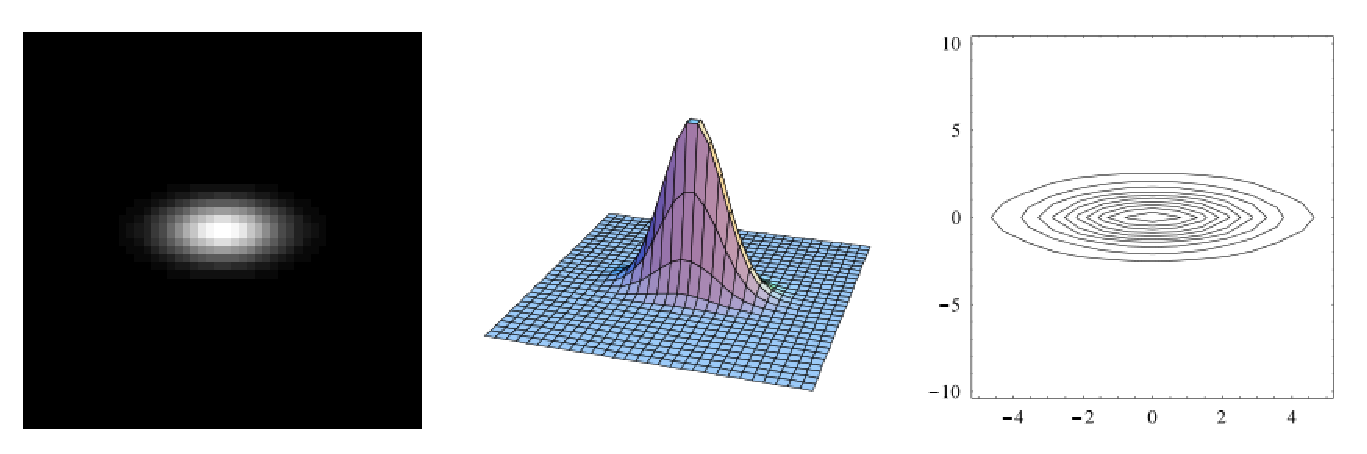
\includegraphics[height=2.2cm,
    angle=0]{./images/Anisotropic_Gaussian.eps}}
\caption{(A) Density Plot; (B) Plot 3D; (C) Contour Plot}
\label{fig:Anisotropic_Gaussian}
\end{figure}

\begin{verbatim}
sx = 2; sy = 1; 
Block[
  {$DisplayFunction = Identity},
  p1 =
     DensityPlot[gauss[x, y, sx, sy], {x, -10, 10}, {y, -10, 10}, 
                 PlotPoints -> 50]; 
  p2 = Plot3D[gauss{x, y, sx, sy}, {x, -10, 10}, {y, -10, 10}, Shading -> True];
  p3 = ContourPlot[gauss{x, y, sx, sy}, {x, -5, 5}, {y, -10, 10}]
  ];
Show[GraphicsArray[{p1, p2, p3}], ImageSize -> 500];
\end{verbatim}


\subsection{Fourier transform}

The purpose of Fourier transform is to identify some periodic behavior in the
data, i.e. using spectral analysis. IDL provides an intrinsic function {\bf
FFT()}\footnote{\url{http://www.ratsimandresy.org/IDL/FFT/}}
\begin{verbatim}
result = FFT(series)
\end{verbatim} 
For digital signals, DFT is the most widely used method for determining the
frequency spectra of digital signals. FFT is the efficient algorithm to do DFT.
FFT convert an image into sines and cosines of different amplitudes and phases.
Then the resulted image in frequency domain can tell how often patterns are
repeated within an image. There are two types of frequencies
\begin{enumerate}
  \item low frequencies: represent gradual variations in the original image
  (and thus tend to contain most information). It's shown as a large peak in the
  center of the frequency-domain data (brightest pixels). If it's shown as a
  surface, the peak shown as a spike. 
  
  \item high frequencies: represent abrupt variations in the original image
  (provide detail in the image, and thus is sensitive to noise which is
  typicall result in abrupt change in spatial data)
  
\end{enumerate}
Depending on what aspect we want to study, we can apply low-pass filter or
high-pass filter to select which frequencies to analyze. For example: we remove
the high frequencies, and then revert back the low-frequencies component to
spatial domain; we then have the new image in which the noise has been removed.


To generate pseudo-linescan image, typically you need to do convolution of the
generated data and the point-spread function (PSF). The convenient, more
computational efficient way is to map both function to the Fourier domain, where
the convolution operation is mapped to multiplication which is easier to carry
out. To obtain the line-scan image, we do inverse Fourier transformation on the
output. 

In Fourier domain, the basis functions are the sinusoidal functions
$\exp\{i\omega x\}$. Given a function f(x), the Fourier transform maps f(x) to
F($\omega$)
\begin{equation}
F(\omega) = \mathcal{F}(f(x)) = \frac{1}{2\pi}\int^\infty_{-\infty}
f(x)e^{i\omega x} dx
\end{equation}
The integration is an intrinsic function in Mathematica.

\subsection{Noise}
\label{sec:noise_confocalmicroscopy}

Remember that to capture an image, the line, reflected on the object, passing
through a small hole (pinhole camera) and projected an inverted image on the opposite side of the
box. The pinhole in human eye is the pupil. 

The smaller the pinhole, the sharper the image, but the dimmer the projected
image. In the camera, this can be adjusted via the so-called {\bf aperture}.
Ideally, the size of the aperture should be 1/100 or less of the distance from
the object to the projected image. Similarly, different confocal microscopies
use different ``optimum diameter'' for the pinhole \citep{sheppard1992}.

\subsection{-- Single photon fluorescence microscopy}

\begin{framed}
wide-field microscope is a type of confocal microscope where the entire
fluorescent specimen is imaged, where also the secondary fluorescence emitted by
the specimen interfere with the signal in focus. As a result, it may cause a
problem for specimens having the thickness of greater than 2$\mum$. Because of
this lack of resolution, the Nyquist rate is about double of that, i.e.
1$\mum$ \footnote{\url{http://www.svi.nl/WideFieldMicroscope}}.

Nyquist sampling spacing is $v_n=\pi/2$. The first zero of Airy disk occurs at
$v=3.83$. So, Nyquist sampling spacing is $v_n=\pi/(2*3.83)=1$AU/2.44. So, the
sampling should be lower or equal to Nyquist spacing.  
\end{framed}

The signal-to-noise in confocal microscopy is often low. Especially due to
fluorophore bleaches after exposing to light, thus limiting the total number of
photons that can be detected by the microscopy. As the number of particles (the
photon) that carry energies is sufficient small, the noise
(uncertainties) is due to Poisson distribution. When the number of photons is
higher, the distribution tends to symmetric, and becoming similar to Gaussian
distribution. Thus making shot noise in actual observation indistinguishable from true
Gaussian noise. 

The mean of a Poisson distribution is equal to its variance. The noise is given
by the square root of the vaiance of the shot noise on a signal of $n_p$
photons, i.e.

\begin{verbatim}	
SNR = sqrt(n_p)
\end{verbatim}

A beam light of power $p$ incident for a time $t$ contains $n_p$ photons.
\begin{equation}
n_p = \frac{Pt\lambda}{hc}
\end{equation}
with $c=2.998\times 10^8$ (m.s$^{-1}$) is velocity of light, $c=\nu \lambda $.
Each photon contains an energy $h\nu$ (where $h=6.626\times 10^{-34}$ (J.s) is
Planck's constant) and $\nu$ is the frequency.

Suppose the light is detected by a photon-detector of quantum efficiency $Q_p$
(the fraction of photons detected by the detector). If the detector also
contribute a sensor noise of $n_n$ electrons, then the SNR becomes
\begin{equation}
SNR = \frac{Q_En_p}{\sqrt{Q_En_p+n^2_n}}
\end{equation}

When the background noise (stray light $N_1$) $n_pB_{N1}$ is considered using
the assumption that background noise is uniformly distributed through the
pinhole, i.e. the intensity is proportional to the area: $B_{N1}=av^2_d/4$, with
$a$ is a constant, $v_d$ is radius of the detector in normalized coordinates
\begin{equation}
v_d = (2\pi r_d/\lambda)\sin \alpha_d
\end{equation} 
So, the SNR is now
\begin{equation}
SNR =
\frac{Q_En_pF(v_d)}{\sqrt{Q_En_p\left[F(v_d)+av^2_d/4+B_{N2}(v_d)\right]+n^2_n}}
\end{equation}
For a square detector, e.g. CCD, the fraction of signal light incident on the
pinhole then $F(v_d)\approx v^2_d/\pi$.

So, the number of perceived gray levels is $g$
\begin{equation}
g = 1 + SNR
\end{equation} 

\subsection{-- Multi-photon fluorescence microscopy}

Using 2 or 3 photon system, the SNR can be calculated similar to above section.
The SNR is best at pinhole radius 0.63 Airy units ($v_d=2.42$) for 2-photon
system, and 0.64 Airy units ($v_d=2.44$) for 3-photon fluorescence. This best
value is 1.6 and 1.9 for 2-photon and 3-photon system, respectively
\citep{sheppard2006}.


For a detector with elements each of length $2v_d$, to achieve Nyquist sampling
$v_d=\pi/4$ (in optical units, e.g. pixels). So, if there are $n$ samples in an
1D image, the field of view is $2v_s=n\pi/2$.

\section{Immunostaining}
\label{sec:immunostaining}

Immunostaining refers to the use of an antibody-based method to detect a specific protein in a sample. 
Here, antibodies labelled with heavy metal particles (e.g. gold), or known as
imm can be directly visualised using transmission electron microscopy.
